\documentclass[12pt]{article}
\usepackage{preamble}

\pagestyle{fancy}
\fancyhead[LO,LE]{Специальные разделы \\ высшей математики}
\fancyhead[RO,RE]{Лекции Далевской О. П.}

\renewcommand{\thesection}{}

\begin{document}

    \tableofcontents
    \clearpage

    
    \section{1. Евклидовы пространства}


    \section{1.1. Скалярное произведение}

    $L$ - линейное пространство $\quad \forall x, y \in L \ \unserset{c = (x, y) - \text{ск. произв.}}{x, y \to c \in \Real}$

    \begin{enumerate}
        \item $(x, y) = (y, x)$
        \item $(\lambda x, y) = \lambda (x, y), \quad \lambda \in \Real$
        \item $(x + z, y) = (x, y) + (z, y)$
        \item $\forall x \in L\ (x, x) \geq 0$ и $(x, x) = 0 \Longrightarrow x = 0$
    \end{enumerate}

    Если векторы и коэффициенты комплескно-значные, то определения будут другими

    \Def Скалярная функция $c = (x, y)$ со свойствами 1-4 называется скалярным произведением элементов $x$ и $y$

    \Def Линейное пространство со скалярным произведением называется \underline{Евклидовым}

    \ExN{1} ЛП - пространство геометрических векторов

    $(\overrightarrow{a}, \overrightarrow{b}) =
    \begin{sqcases}
        |\overrightarrow{a}||\overrightarrow{b}|\cos\varphi, \quad \overrightarrow{a}, \overrightarrow{b} \neq 0 \\
        0, \quad \overrightarrow{a} = 0 \lor \overrightarrow{b} = 0
    \end{sqcases}$

    \ExN{2} ЛП $\displaystyle = C_{[a;b]}$

    $\displaystyle (f(x), g(x)) \stackrel{def}{=} \int^b_a f(x)g(x) dx$

    Очевидно, что 1-3 выполняются, проверим 4:

    $\displaystyle \int^b_a f^2(x) dx = 0 \stackrel{?}{\Longrightarrow} f(x) = 0$

    \ExN{3} ЛП - пространство числовых строк вида $\displaystyle x = (x_1, x_2, \dots, x_n)$

    $\displaystyle (x, y) = x_1 y_1 + \dots x_n y_n = \sum_{i=1}^n x_i y_i$ - сумма произведений компонент

    \section{1.2. Свойства евклидова пространства - $E$}

    \Th Неравенство Коши-Буняковского

    $\displaystyle (x, y)^2 \leq (x, x)(y, y)$

    $\Box$

    Нетрудно заметить, что:

    $\displaystyle \sphericalangle (\lambda x - y, \lambda x - y) = (\lambda x - y, \lambda x) - (\lambda x - y, y) =
    (\lambda x, \lambda x) - (y, \lambda x) - (\lambda x, y) + (y, y) = \lambda^2 (x, x) - 2\lambda (x, y) + (y, y) \stackrel{\text{пусть}}{=} 0$

    Решим относительно $\lambda$

    $\displaystyle D = 4(x, y)^2 - 4(x, x)(y, y)$

    $\displaystyle \frac{D}{4} = (x, y)^2 - (x, x)(y, y)$

    Так как $(\lambda x - y) \geq 0$ (4-ое свойство ск. произв.), то уравнение имеет $\leq 1$ корня, значит
    $\displaystyle \frac{D}{4} = (x, y)^2 - (x, x)(y, y) \leq 0$

    $\Box$

    \section{1.3. Норма}

    ЛП $= L, \forall x \in L$ определена функция так, что выполняется $x \to n \in \Real, n = \|x\|$

    \begin{enumerate}
        \item $\|x\| \geq 0$ и $\|x\| = 0 \Longrightarrow x = 0$
        \item $\|\lambda x\| = |\lambda| \cdot \|x\| \quad \lambda \in \Real$
        \item $\|x + y\| \leq \|x\| + \|y\| \quad \forall x, y \in L$
    \end{enumerate}

    Евклидово пространство с нормой называется нормированным

    \Th $\displaystyle E^n$ является нормированным, если $\|x\| = \sqrt{(x, x)}$

    $\Box$

    Свойства 1-2 очевидны, докажем 3 свойство:

    $\|x + y\| = \sqrt{(x + y, x + y)} \leq \sqrt{(x, x)} + \sqrt{(y, y)} = \|x\| + \|y\|$

    $\sqrt{(x, x) + 2(x, y) + (y, y)} \leq \sqrt{(x, x)} + \sqrt{(y, y)}$

    $(x, x) + 2(x, y) + (y, y) \leq (x, x) + (y, y) + 2\sqrt{(x, x)(y, y)}$

    $(x, y) \leq \sqrt{(x, x)(y, y)}$

    $\displaystyle (x, y)^2 \leq (x, x)(y, y)$ - верно по неравенству Коши-Буняковского

    $\Box$

    Обобщим геометрические понятия ортогональности и косинуса угла на случай произвольных векторов

    \Def $x, y$ - ортогональны, если $(x, y) = 0$ и $x \neq 0$ и $y \neq 0 \quad x \perp y$

    \Def $\displaystyle \cos(\widehat{x, y}) = \frac{(x, y)}{\|x\|\cdot\|y\|}$ - косинус угла между векторами

    \Def $\displaystyle x, y \in E^n \quad x \perp y \quad z = x + y$ - гипотенуза

    \Th $x \perp y$, тогда $\displaystyle \|x + y\|^2 = \|x\|^2 + \|y\|^2$

    $\Box$

    $\displaystyle \|x + y\|^2 = (x + y, x + y) = (x, x)^2 + \underset{= 0, x \perp y}{\undergroup{2(x, y)}} + (y, y)^2 = (x, x)^2 + (y, y)^2$

    $\Box$

    \Def $\displaystyle B = \Set{e_i}_{i=1}^n$ - базис $\displaystyle L^n$

    На $\displaystyle L^n$ введены $(x, y)$ и $\|x\|$ (то есть $\displaystyle L^n \to E^n_{\|\cdot\|}$ - нормированное евклидово)

    $B$ называют ортонормированным базисом, если $\displaystyle (e_i, e_j) = \begin{cases}0, i \neq j \\ 1, i = j\end{cases}$

    \Nota Докажем, что всякая такая система из $n$ векторов линейно независима (то есть всякая нулевая комбинация тривиальная):

    $\displaystyle \sum_{i=1}^n \lambda_i e_i = 0 \stackrel{?}{\Longrightarrow} \forall \lambda_i = 0$

    $\displaystyle (e_k, \sum_{i=1}^n \lambda_i e_i) = \sum_{i=1}^n \lambda_i (e_k, e_i) \stackrel{k \neq i \Rightarrow (e_k, e_i) = 0}{=\joinrel=\joinrel=}
    \lambda_k \|e_k\|^2 = \lambda_k = 0 \quad \forall k$



    \textit{(записи внезапно обрываются)}



    \Nota Изоморфизм $\displaystyle E^n \rightarrow E^{\prime n}$ позволяет переносить свойства скалярного произведения
    из одного в другое пространство

    Ex: $\|x + y\| \leq \|x\| + \|y\|$ - арифметические векторы со скалярным произведением $\displaystyle (x, y) = \Sigma^n_{i=1} x_i y_i$

    $\displaystyle E^{\prime n} \in C_{[a;b]}$ со скалярным произведением $\displaystyle (f, g) = \int^b_a f * g dx$

    $\displaystyle \sqrt{\int^b_a (f * g)^2 dx} \leq \sqrt{\int^b_a f^2 dx} + \sqrt{\int^b_a g^2 dx}$

    \textbf{Задача о перпендикуляре}

    Постановка: Нужно опустить перпендикуляр из точки пространства $\displaystyle E^n$ на подпространство $G$

    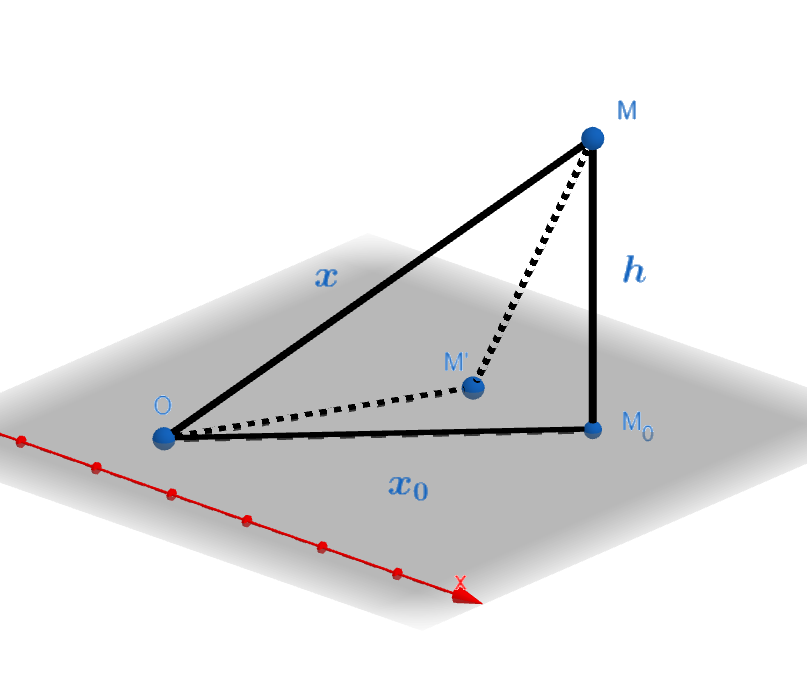
\includegraphics[height=90mm]{images/specsec_2024_03_01_1}

    Точка $M$ - конец вектора $x$ в пространстве $\displaystyle E^n$.
    Нужно найти $\displaystyle M_0$ (конец вектора $\displaystyle x_0$, проекции $x$ на $G$)

    \[x_0 + h = x\]

    где $h \perp G$. Правда ли что, длина перпендикулярного вектора $h$ - минимальная длина от точки $M$ до $G$?

    \Th $\displaystyle h \perp G, x_0 \in G, x = x_0 + h$. Тогда $\displaystyle \forall x^\prime \in G (x^\prime \neq x_0) \ \ \|x - x^\prime\| > \|x - x_0\|$

    $\displaystyle \Box \|x - x^\prime\| = \|x - x_0 + x_0 - x^\prime\| \stackrel{\text{по теореме Пифагора}}{====} \|x - x_0\| + \|x_0 - x^\prime\| = \|h\| + \|x_0 - x^\prime\| > \|x - x_0\|$

    \Nota $\displaystyle x_0$ называется ортогональной проекцией, возникает вопрос о ее вычислении (так находятся основания перпендикуляров)

    \vspace{5mm}

    \textit{Алгоритм:} $\displaystyle x_0 = \lambda_1 e_1 + \lambda_2 e2 + \dots + \lambda_k + e_k$, $\displaystyle \{e_i\}^k_{i=1}$ - базис $G$ (необязательно ортонормированный)

    Дан вектор $x$, пространство $G$, нужно найти $\displaystyle \lambda_i$

    $\displaystyle h = x - x_0$, $\displaystyle h \perp G \quad  (h, e_i) \stackrel{h \perp e_i \ \forall i}{=} 0$

    $\displaystyle (x - x_0, e_i) = (x, e_i) - (x_0, e_i) = 0$

    $\displaystyle (x, e_i) = (x_0, e_i)$

    Тогда $\displaystyle \forall i \quad (x_0, e_i) = (\lambda_1 e_1 + \dots + \lambda_k e_k, e_i) = \lambda_1 (e_1, e_i) + \dots + \lambda_k (e_k, e_i)$ - $\displaystyle (e_k, e_i)$ - числа, а $\displaystyle \lambda_i$ - неизвестные

    Получили СЛАУ:

    $\displaystyle \begin{array}{|cccc|}
    (e_1, e_1) & (e_1, e_2) & \ldots & (e_1, e_k)\\
    \ldots & \ldots & \ldots & \ldots\\
    (e_k, e_1) & (e_k, e_2) & \ldots & (e_k, e_k)\\
    \end{array} \times \begin{array}{|c|}
    \lambda_1\\
    \ldots\\
    \lambda_k \\
    \end{array} = \Gamma \times \begin{array}{|c|}
    \lambda_1\\
    \ldots\\
    \lambda_k \\
    \end{array} = \begin{array}{|c|}
    (x,e_1)\\
    \ldots\\
    (x,e_k) \\
    \end{array}$

    \Nota В матрице $\Gamma$ нет нулевых строк, так как $\displaystyle e_i$ - бизисная и по крайней мере $\displaystyle e_i^2 \neq 0$

    Таким образом по теореме Крамера $\displaystyle \exists! (\lambda_1, \dots, \lambda_k)$

    \Def Матрица $\displaystyle \Gamma = {(e_i, e_j)}_{i, j = 1\dots k}$ называют матрицей Грама

    $\Gamma = I = \begin{array}{|ccc|}
    1 & 0 & \ldots\\
    0 & 1 & \ldots\\
    \ldots & \ldots & 1\\
    \end{array}$, если базис ортонормированный

    Далее, $I$ - единичная матрица Грама

    \Nota Тогда $\displaystyle I \times \begin{array}{|c|}
    \lambda_1\\
    \ldots\\
    \lambda_k \\
    \end{array} = \begin{array}{|c|}
    \lambda_1\\
    \ldots\\
    \lambda_k \\
    \end{array} = \begin{array}{|c|}
    (x,e_1)\\
    \ldots\\
    (x,e_k) \\
    \end{array}$

    \vspace{5mm}

    \textbf{Приложения задачи о перпендикуляре}

    1) Метод наименьших квадратов

    В качестве простейшей модели зависимости $y = y(x)$ берем линейную функцию $y = \lambda x$

    Ищем минимально отстоящую прямую от данных $\displaystyle (x_i, y_i)$, то есть ищем $\lambda$

    Определим расстояние (в этом методе) как $\displaystyle \sigma^2 = \Sigma^n_{i=1} (y_i - y_{0i})^2 = \Sigma^n_{i=1} (y_i - \lambda x_i)^2$ - минимизируем

    Таким образом, ищем $\displaystyle y_0$ (ортог. проекция) такое, что $\displaystyle (y - y_0)^2 = \sigma^2$ - минимальное

    Если $\displaystyle y_0 = \lambda_1 x_1 + \dots + \lambda_k x_k$, где $\displaystyle x_i$ - набор измерений для $i$-ой точки

    Рассмотрим $\displaystyle y_0$ как разложение по базису $\displaystyle \{x_i\}$

    \vspace{5mm}

    2) Многочлен Фурье

    $\displaystyle P(t) = \frac{a_0}{2} + a_1 cos t + b_1 sin t + \dots a_n cos nt + b_n sin nt$ - линейная комбинация

    Функции ${1, cos t, sin t, \dots, cos nt, sin nt}$ - ортогональны

    Задача в том, чтобы для функции $f(t)$, определенной на отрезке $[0;2\pi]$ найти минимально отстоящий многочлен $P(t)$ при том,
    что расстояние определяется как $\displaystyle \sigma^2 = \int_0^{2\pi} (f(t) - P(t))^2 dt$

    Нужно найти $\displaystyle a_i$ и $\displaystyle b_i$ - обычные скалярные произведения $\displaystyle a_i = k \int_0^{2\pi} f(t) cos(it) dt$, $\displaystyle b_i = m \int_0^{2\pi} f(t) sin(it) dt$ ($k, m$ - нормирующие множители)

    \clearpage

    \section{2. Линейный оператор (линейное отображение, линейный функционал, линейное преображение)}

    \section{2.1. Определение}

    \textit{Линейный оператор} - это отображение $\displaystyle V^n \stackrel{\mathcal{A}}{\Longrightarrow} W^m$

    ($\displaystyle V^n, W^m$ - линейные пространства размерности $n \neq m$ в общем случае),

    которое $\displaystyle \forall x \in V^n$ сопоставляет один какой-либо $\displaystyle y \in W^m$ и

    $\displaystyle \mathcal{A} (\lambda x_1 + \mu x_2) = \lambda \mathcal{A} x_1 + \mu \mathcal{A} x_2 = \lambda y_1 + \mu y_2$

    \Nota Заметим, что если 0 представим как $0 * x$, где $x \neq 0$, то

    $\mathcal{A}(0) = \mathcal{A}(0 * x) = 0 * \mathcal{A}x \stackrel{0 * y}{=} 0$

    \Nota Если $V = W$, то $\mathcal{A}$ называют линейным преобразованием, но далее будем рассматривать в основном операторы $\mathcal{A}: \ \ V \rightarrow V$, $\displaystyle \mathcal{A}: \ \ V^n \rightarrow W^n$



    \ExN{1} $\displaystyle V = \Real^2$ - пространство направленных отрезков

    $\mathcal{A}: V \leftarrow V$

    $\displaystyle \mathcal{A}x = y = \lambda y_1 + \mu y_2$ для таких $\mathcal{A}$ как сдвиг, поворот, гомотетия, симметрия

    \ExN{2} $\displaystyle V^n = W^m$, где $m < n$

    $\mathcal{A}$ - оператор проектирования (убедиться, что он линейный)

    \ExN{3} $\displaystyle V^n$ - пространство числовых строк длины $n$

    $\displaystyle \mathcal{A}: V^n \leftarrow V^n$

    $\displaystyle x = (x_1, \dots, x_n), y = (y_1, \dots, y_n)$

    $\displaystyle \mathcal{A}x = y : \begin{array}{|ccc|}
    a_{11} & \ldots & a_{1n}\\
    \vdots & \ddots & \vdots\\
    a_{n1} & \ldots & a_{nn}\\
    \end{array}x = y$


    \section{2.2. Действия с операторами}

    \Def $\mathcal{A}\mathcal{B}: V \rightarrow W$

    \begin{enumerate}
        \item $(\mathcal{A} + \mathcal{B})x \stackrel{def}{=} \mathcal{A}x + \mathcal{B}x$ - определение суммы $\mathcal{A} + \mathcal{B} = \mathcal{C}$
        \item $(\lambda\mathcal{A})x \stackrel{def}{=} \lambda(\mathcal{A}x)$ - $\lambda\mathcal{A} = \mathcal{D}$
    \end{enumerate}

    \Nota Сформируем линейное пространство из операторов $\mathcal{A}: V \rightarrow W$

    \begin{enumerate}
        \item Ассоциативность сложения (очевидно)
        \item Коммутативность (очевидно)
        \item Нейтральный элемент $\mathcal{O}x = 0$
        \item Противоположный: $-\mathcal{A} = (-1) * A$
        \item \dots \textit{LAB}
    \end{enumerate}

    \textit{Def:} $\mathcal{I}$ - тождественный - $\forall x \in V \ \ \mathcal{I}x = x$



    \Def Произведение операторов (композиция)

    $\mathcal{A}\mathcal{B}$ - произведение, $\mathcal{A} : V \rightarrow W; \ \mathcal{B} : U \rightarrow V$

    $(\mathcal{A}\mathcal{B}) x = \mathcal{A}(\mathcal{B}x); \quad x \in U$

    Свойства: \underline{Lab} доказать

    1* $\lambda (\mathcal{A}\mathcal{B}) = (\lambda \mathcal{A})\mathcal{B}$

    2* $(\mathcal{A} + \mathcal{B}) \mathcal{C} = \mathcal{A}\mathcal{C} + \mathcal{B}\mathcal{C}$

    3* $\mathcal{A} (\mathcal{B} + \mathcal{C}) = \mathcal{A}\mathcal{B} + \mathcal{A}\mathcal{C}$

    4* $\mathcal{A} (\mathcal{B}\mathcal{C}) = (\mathcal{A}\mathcal{B}) \mathcal{C}$


    \Nota Можно обобщить 4* на $n$ равных $\mathcal{A}$

    \Def $\displaystyle \mathcal{A}^n = \mathcal{A} \cdot \mathcal{A} \dots \mathcal{A}$ - $n$ раз, степень оператора

    Свойства: $\displaystyle \mathcal{A}^{m + n} = \mathcal{A}^n \cdot \mathcal{A}^m$

    \section{2.3. Обратимость оператора}

    Def: $\mathcal{A} : V \rightarrow W$ так, что $\mathcal{A}V = W$ и $\displaystyle \forall x_1 \neq x_2 (x_1, x_2 \in V) \quad
    \begin{cases}y_1 = \mathcal{A}x_1 \\ y_2 = \mathcal{A}x_2\end{cases} \Longrightarrow y_1 \neq y_2$

    Тогда $\mathcal{A}$ называется взаимно-однозначно действующим

    Nota: Проще сказать \enquote{линейный изоморфизм}

    \Th $\displaystyle \Set{x_i}$ - линейно независима $\displaystyle \stackrel{\mathcal{A}x = y}{\longrightarrow} \Set{y_i}$ - линейно независима

    В обратную сторону, если $\mathcal{A}$ - взаимно-однозначен

    $\Box \sqsupset \mathcal{A} : V \rightarrow W$ и $\displaystyle \texttt{0}_V, \texttt{0}_W$ - нули $V$ и $W$ соответственно
    \begin{enumerate}
        \item $\displaystyle \mathcal{A}(\texttt{0}_V) = \mathcal{A}(\Sigma^k_{i=1} 0 \cdot e_i) = \Sigma^k_{i=1} 0 \cdot \mathcal{A}e_i = \texttt{0}_W$

        \item Докажем, что если $\displaystyle {x_i} \subset V$ - лин. нез., то $\displaystyle {y_i} \subset W$ - лин. нез.

        Составим $\displaystyle \Sigma^m_{j=1} \lambda_j y_j = \texttt{0}_W$ (От противного) $\displaystyle \sqsupset \Set{y_i}$ - лин. зав., тогда $\displaystyle \exists \lambda_k \neq 0$

        При этом $\displaystyle \forall j \ \ y_j = \mathcal{A}x_j$ (т. к. $\mathcal{A}$ - вз.-однозн., то $\displaystyle n^\prime = m^\prime$: кол-во $\displaystyle x_i$ и $\displaystyle y_i$ равно)

        $\displaystyle \Sigma^m^\prime_{j=1} \lambda_j \mathcal{A}x_j \stackrel{\text{линейность}}{=} \mathcal{A} (\Sigma^m^\prime_{j=1} \lambda_j x_j) = \texttt{0}_W$

        Так как $\displaystyle \mathcal{A}\texttt{0}_V = \texttt{0}_W$, то $\displaystyle \texttt{0}_W$ - образ $\displaystyle x = \texttt{0}_V$, но так как $\mathcal{A}$ - вз.-однозн., то
        $\displaystyle \nexists x^\prime \neq x \ | \ \mathcal{A}(x^\prime) = \texttt{0}_W$

        Значит $\displaystyle \Sigma^m^\prime_{j=1} \lambda_j x_j = \texttt{0}_V$, но $\displaystyle \exists \lambda_k \neq 0 \Longrightarrow \Set{x_j}$ - лин. зав. - \underline{противоречие}

        \item $\sqsupset$ теперь $\displaystyle \Set{y_i}$ - л. нез., а $\displaystyle \Set{x_i}$ (по предположению от противного) - лин. зав.

        $\displaystyle \Sigma^{n^\prime}_{i = 1} \lambda_i x_i \stackrel{\exists \lambda_k \neq 0}{=} \texttt{0}_V \quad \Big| \mathcal{A}$

        $\displaystyle \Sigma^{n^\prime}_{i = 1} \lambda_i \mathcal{A}x_i = \texttt{0}_W$

        При этом $\displaystyle \exists \lambda_k \neq 0 \Longrightarrow \Set{y_i}$ - лин. зав. - \underline{противоречие}

    \end{enumerate}

    Следствие: $\dim V = \dim W \Longleftarrow \mathcal{A}$ - лин. изоморфизм

    Def: $\mathcal{B} : W \rightarrow V$ называется обратным оператором для $\mathcal{A} : V \rightarrow W$

    если $\mathcal{B}\mathcal{A} = \mathcal{A}\mathcal{B} = \mathcal{I}$ (обозначается $\displaystyle \mathcal{B} = \mathcal{A}^{-1}$)

    Следствие: $\displaystyle \mathcal{A}\mathcal{A}^{-1} x = x$

    \Th $\mathcal{A}x = \texttt{0}$ и $\displaystyle \exists \mathcal{A}^{-1}$, тогда $x = \texttt{0}$

    $\displaystyle \Box \mathcal{A}^{-1}\mathcal{A} x = \mathcal{A}^{-1}(\mathcal{A} x) = \mathcal{A}^{-1} \texttt{0}_W = \texttt{0}_V \Longrightarrow x = \texttt{0}$

    \Th Н. и Д. условия существования $\displaystyle \mathcal{A}^{-1}$

    $\displaystyle \exists \mathcal{A}^{-1} \Longleftrightarrow \mathcal{A}$ - вз.-однозн.

    $\displaystyle \Box \Longrightarrow \exists \mathcal{A}^{-1}$, но $\sqsupset \mathcal{A}$ - не вз.-однозн., то есть
    $\displaystyle \exists x_1, x_2 \in V (x_1 \neq x_2) \ | \ \mathcal{A}x_1 = \mathcal{A}x_2 \Longleftrightarrow \mathcal{A}x_1 - \mathcal{A}x_2 = \texttt{0} \Longleftrightarrow
    \mathcal{A}(x_1 - x_2) = \texttt{0}_W \stackrel{\exists \mathcal{A}^{-1}}{\Longrightarrow} x = \texttt{0}_V \Longleftrightarrow x_1 = x_2$ - противоречие

    $\Longleftarrow$ Так как $\mathcal{A}$ - изоморфизм (не учитывая линейность), то $\displaystyle \exists \mathcal{A}^\prime$ - обратное отображение (не обязат. линейное)

    Докажем, что $\displaystyle \mathcal{A}^\prime : W \rightarrow V$ - линейный оператор

    ? $\displaystyle \mathcal{A}^\prime (\Sigma \lambda_i y_i) = \Sigma \lambda_i \mathcal{A}^\prime y_i = \Sigma \lambda_i x_i$

    $\mathcal{A}$ - вз.-однозн. $\displaystyle \Longleftrightarrow \forall x_i \longleftrightarrow y_i \quad \Big| \cdot \lambda_i, \Sigma$

    $\displaystyle \mathcal{A}(\Sigma \lambda_i x_i) = \mathcal{A} x = y = \Sigma \lambda_i y_i \quad$ и $y$ имеет только один прообраз $x$

    Применим $\displaystyle \mathcal{A}^\prime$ к $\displaystyle y = \Sigma \lambda_i y_i \quad \mathcal{A}^\prime y = x = \Sigma \lambda_i x_i$ - единственный прообраз $y$

    Таким образом, $\displaystyle \mathcal{A}^\prime$ переводит лин. комбинацию в такую же лин. комбинацию прообразов, то есть $\displaystyle \mathcal{A}^\prime$ - линейный: $\displaystyle \mathcal{A}^\prime = \mathcal{A}^{-1}$

    \section{2.4. Матрица ЛО}

    $\displaystyle \mathcal{A} : V^n \rightarrow W^m$

    Возьмем вектор $\displaystyle x \in V^n$ и разложим по какому-либо базису $\displaystyle \Set{e_j}^n_{j=1}$

    $\displaystyle \mathcal{A}x = \mathcal{A} (\Sigma^n_{j=1} c_j e_j) = \Sigma^n_{j=1} c_j \mathcal{A}e_j$

    $\displaystyle \mathcal{A} e_j \stackrel{\text{образ базисного вектора}}{=} y_j \stackrel{\Set{f_i} - \text{ базис } W^m}{=} \Sigma^m_{i=1} a_{ij}f_i$

    $\displaystyle \mathcal{A}x = \Sigma^n_{j=1} c_j \mathcal{A}e_j = \Sigma^n_{j=1} c_j \Sigma^m_{i=1} a_{ij}f_i = \Sigma^n_{j=1} \Sigma^m_{i=1} c_j a_{ij} f_i = \Sigma^m_{i=1} \Sigma^n_{j=1} c_j a_{ij} f_i$

    Иллюстрация:

    $\displaystyle \begin{pmatrix}
         a_{11} & \dots & a_{1n} \\
         \vdots & \ddots & \vdots \\
         a_{m1} & \dots & a_{mn} \\
    \end{pmatrix} \begin{pmatrix}
         c_{1} \\
         \vdots \\
         c_{n} \\
    \end{pmatrix} = \begin{pmatrix}
         b_{1} \\
         \vdots \\
         b_{m} \\
    \end{pmatrix}$

    Def: Матрица $\displaystyle A = {a_{ij}}_{i=1..m, j=1..n}$ называется матрицей оператора $\displaystyle \mathcal{A} : V^n \rightarrow W^m$ в базисе $\displaystyle \Set{e_j}^n_{j=1}$ пространства $\displaystyle V^n$

    Вопросы:

    1) $\forall ? \mathcal{A} \ \exists A$

    2) $\forall ? A \ \exists \mathcal{A}$

    3) если $\exists A$ для $\mathcal{A}$, то единственная?

    4) если $\exists \mathcal{A}$ для $A$, то единственная?

    Ответы:

    1) При выбранном базисе $\displaystyle \Set{e_j} \ \forall \mathcal{A} \ \exists A$ (алгоритм выше)

    3) такая $A$ единственная $\Longrightarrow$ в разных базисах матрицы ЛО $\displaystyle \mathcal{A} \quad A_e \neq A_{e^\prime}$

    2) $\displaystyle \forall A_{m\times n}$ можно взять пару ЛП $\displaystyle V^n, W^m$ и определить $\displaystyle \mathcal{A} : V^n \rightarrow W_n$ по правилу $\displaystyle \mathcal{A}e_V = e_W^\prime$

    4) \Lab

    Nota: Далее будем решать две задачи

    1) преобразование координат как действие оператора

    2) поиск наиболее простой матрицы в некотором базисе

    \section{2.5. Ядро и образ оператора}

    \Def Ядро оператора - $\displaystyle Ker \mathcal{A} \stackrel{def}{=} \Set{x \in V \ | \ \mathcal{A}x = \texttt{0}_W}$

    \Def Образ оператора - $Im \mathcal{A} \stackrel{def}{=} \Set{y \in W \ | \ \mathcal{A}x = y}$

    \Nota $Ker \mathcal{A}$ и $Im \mathcal{A}$ - подпространства



    \Nota $Ker\ \mathcal{A}$ и $Im\ \mathcal{A}$ - подпространства $V$ ($\mathcal{A} : V \rightarrow V$)

    Вообще-то $Ker\ \mathcal{A} \subset V, Im\ \mathcal{A} \subset W \ (\mathcal{A} : V \rightarrow W)$

    $\dim W \leq \dim V$, тогда можно считать, что $\displaystyle W \subset V^\prime$ и
    рассмотрим $\displaystyle \mathcal{A} : V \rightarrow V^\prime$ (где $\displaystyle V^\prime$ изоморфен $V$)

    $Ker \mathcal{A}$ - подпространство, то есть $Ker \mathcal{A} \subset V$ и
    $\displaystyle \Sigma c_i x_i \subset \mathcal{A}$, если $\displaystyle \forall x_i \in Ker \mathcal{A}$

    $\displaystyle \mathcal{A} (\Sigma c_i x_i) = \Sigma c_i \mathcal{A} x_i \stackrel{x_i \in \mathcal{A}}{=} \Sigma c_i \texttt{0} = \texttt{0}$

    Следствие: $Ker \mathcal{A} = \texttt{0} \Longrightarrow \mathcal{A}$ - вз.-однозн.

    $\Box$ От противного:

    $\sqsupset \mathcal{A}$ - не вз.-однозн., то есть $\displaystyle \exists x_1, x_2 \in V (x_1 \neq x_2) | \mathcal{A}x_1 = \mathcal{A}x_2 \Longleftrightarrow \mathcal{A} (x_1 - x_2) = \texttt{0} \Longrightarrow x_1 - x_2 \in Ker \mathcal{A}$ - противоречие

    \Nota Обратное также верно:

    $\mathcal{A}$ - вз.-однозн. $\displaystyle \Longleftrightarrow y_1 = y_2 \Longrightarrow x_1 = x_2$, так как $\displaystyle \mathcal{A}(x_1 - x_2) = \texttt{0} \Longrightarrow x_1 - x_2 = 0$

    Тогда $\texttt{0}$ является образом только $\texttt{0}$-вектора $\Longrightarrow Ker \mathcal{A} = \texttt{0}$

    \Nota Также очевидно, что

    $Ker \mathcal{A} = 0 \Longleftrightarrow Im \mathcal{A} = V$

    $Ker \mathcal{A} = V \Longrightarrow Im \mathcal{A} = \texttt{0}$ и $\mathcal{A} = 0$

    \Th $\mathcal{A} : V \rightarrow V$, тогда $\dim Ker \mathcal{A} + \dim Im \mathcal{A} = \dim V$

    $\Box$ Так как $Ker \mathcal{A}$ - подпространство $V$, то можно построить дополнение до прямой суммы (взяв базисные векторы ядра, дополнить их набор до базиса $V$: $\displaystyle e^k_1, \dots e^k_m, e^k_{m+1}, \dots e^k_n$)

    Обозначим дополнение $W$, тогда $Ker \mathcal{A} \xor W = V \Longrightarrow \dim Ker \mathcal{A} + \dim W = \dim V$

    Докажем, что $W$ и $Im \mathcal{A}$ - изоморфны

    $\mathcal{A} : W \rightarrow Im \mathcal{A}$

    $\mathcal{A} : Ker \mathcal{A} \rightarrow \texttt{0}$

    Докажем, что $\mathcal{A}$ действует из $W$ в $Im \mathcal{A}$ взаимно-однозначно

    $\sqsupset \mathcal{A}$ невз.-однозн., тогда $\displaystyle \exists x_1, x_2 \in W (x_1 \neq x_2) | \mathcal{A}x_1 = \mathcal{A}x_2 \in Im \mathcal{A}$

    $\displaystyle \mathcal{A}(x_1 - x_2) = \texttt{0} \Longrightarrow x_1 - x_2 \stackrel{\text{обозн.}}{=} x \in Ker \mathcal{A}$, но $x \neq 0$, так как $\displaystyle x_1 \neq x_2$

    Но для прямой суммы $W \union Ker \mathcal{A} = \texttt{0}, x \ni W \union Ker \mathcal{A} \Longrightarrow$ предположение неверно

    $\Longrightarrow \mathcal{A}$ - лин. вз.-однозн. $\Longrightarrow \dim W = \dim Im \mathcal{A}$

    $\displaystyle V = W_1 \xor W_2$ найдется ЛО $\mathcal{A} : V \rightarrow V$

    $\displaystyle W_1 = Ker \mathcal{A}, W_2 = Im \mathcal{A}$

    \Def Рангом оператора $\mathcal{A}$ называется $\dim Im \mathcal{A}$: $rang \mathcal{A} \stackrel{def}{=} \dim Im \mathcal{A} (= r(\mathcal{A}) = rank \mathcal{A})$

    \Nota Сравним ранг оператора с рангом его матрицы

    $\displaystyle \mathcal{A} x = y \quad \mathcal{A} : V^n \rightarrow W^m$

    $A$ - матрица $\displaystyle \mathcal{A}, x = x_1 e_1 + x_2 e_2 + \dots + x_n e_n, y = y_1 f_1 + \dots + y_m f_m$

    $\displaystyle \mathcal{A}x = y \Longleftrightarrow \begin{pmatrix}
         a_{11} & \dots & a_{1n} \\
         \vdots & \ddots & \vdots \\
         a_{m1} & \dots & a_{mn}
    \end{pmatrix} \begin{pmatrix}
         x_1 \\
         \vdots \\
         x_n
    \end{pmatrix} = \begin{pmatrix}
         y_1 \\
         \vdots \\
         y_m
    \end{pmatrix}$

    Или при преобразовании базиса $\displaystyle Ae_i = e^\prime_i$:

    $\displaystyle \begin{pmatrix}
         a_{11} & \dots & a_{1n} \\
         \vdots & \ddots & \vdots \\
         a_{m1} & \dots & a_{mn}
    \end{pmatrix} \begin{pmatrix}
         e_1 \\
         \vdots \\
         e_n
    \end{pmatrix}^T = \begin{pmatrix}
         e_1^\prime \\
         \vdots \\
         e_m^\prime
    \end{pmatrix}$

    Здесь $\displaystyle \begin{pmatrix}
         e_1 \\
         \vdots \\
         e_n
    \end{pmatrix}^T$ - это матрица $\displaystyle \begin{pmatrix}
         e_1 & \dots & e_n
    \end{pmatrix} = \begin{pmatrix}
         e_{11} & e_{12} & \dots \\
         \vdots & \vdots & \vdots \\
         e_{n1} & e_{n2} & \dots
    \end{pmatrix}$

    \Nota Поиск матрицы $\mathcal{A}$ можно осуществить, найдя ее в \enquote{домашнем} базисе $\displaystyle \Set{e_i}$, то есть $\displaystyle A (e_1, \dots e_n) = (e_1^\prime, \dots, e_m^\prime)$

    Затем, можно найти матрицу в другом (нужном) базисе, используя формулы преобразований (см. \th позже)

    Тогда $Ker \mathcal{A} = K$ - множество векторов, которые решают систему

    $AX = \texttt{0} \quad (\dim K = m = \dim \text{ФСР} = n - rang A)$ и при этом $\dim K = n - \dim Im \mathcal{A}$

    $rang \mathcal{A} = rang A = \dim Im \mathcal{A}$

    Следствия (без док-в)

    1) $rang(\mathcal{AB}) \leq rang(\mathcal{A})$ (или $rang \mathcal{B}$)

    2) $rang(\mathcal{AB}) \geq rang(\mathcal{A}) + rang(\mathcal{B}) - \dim V$

    \Nota Рассмотрим преобразование координат, как линейный оператор $\displaystyle T : V^n \rightarrow V^n$ (переход из системы $\displaystyle Ox_i \rightarrow Ox_i^\prime$, $i = 1..n$)

    $\dim Im T = n, \dim Ker T = 0 \Longrightarrow T$ - вз.-однозн.

    Поставим задачу отыскания матрицы в другом базисе, используя $\displaystyle T_{e \to e^\prime}$

    \section{2.6. Преобразование матрицы оператора при переходе к другому базису}

    \Th $\displaystyle \mathcal{A} : V^n \rightarrow V^n$

    $\displaystyle \Set{e_i} \stackrel{\text{об}}{=} e$ и $\displaystyle \Set{e^\prime_i} \stackrel{\text{об}}{=} e^\prime$ - базисы пространства $V$

    $\displaystyle \mathcal{T} : V^n \rightarrow V^n$ - преобразование координат, то есть $\displaystyle Te_i = e^\prime_i$

    $\displaystyle \sqsupset A, A^\prime$ - матрицы $\mathcal{A}$ в базисах $e$ и $\displaystyle e^\prime$

    Тогда $\displaystyle A^\prime = TAT^{-1}$ ($\displaystyle A^\prime_{e^\prime} = T_{e\to e^\prime}AT^{-1}_{e\to e^\prime}$)

    $\Box \sqsupset y = \mathcal{A}x$, где $x, y$ - векторы в базисе $e$ ($\displaystyle x_e = x^\prime_{e^\prime}$ - один вектор)

    $\displaystyle y^\prime = \mathcal{A} x^\prime$, где $\displaystyle x^\prime, y^\prime$ - векторы в базисе $\displaystyle e^\prime$

    $\displaystyle \mathcal{T}x = x^\prime, \mathcal{T}y = y^\prime$

    $y = Ax$, $\displaystyle y^\prime = A^\prime x^\prime$, тогда $\displaystyle Ty = A^\prime (Tx) \quad \Big| \cdot T^{-1}$

    $\displaystyle T^{-1}Ty = (T^{-1}A^\prime T)x$
    
    $\displaystyle Ax = y = (T^{-1}A^\prime T)x$

    $\displaystyle A = T^{-1}A^\prime T \Longrightarrow A^\prime = TA T^{-1}$



    \Th $\displaystyle A^\prime = T_{e\to e^\prime} A T^{-1}_{e\to e^\prime}$

    \Nota $C = A + \lambda B$

    Следствия:

    1) $\displaystyle TCT^{-1} = T (A + \lambda B) T^{-1} = T A T^{-1} + \lambda T B T^{-1}$

    2) $\displaystyle B = I \quad T B T^{-1} = T I T^{-1} = I$, т. к. $\displaystyle TI = T, T T^{-1} = I$

    3) $\displaystyle \det A^{-1} = \det (T A T^{-1}) = \det T \det A \det T^{-1} = \det A \cdot 1$

    \Nota То есть характеристика нашего объекта - инвариант при преобразовании $T$

    \Def Матрица $A$ называется ортогональной если $\displaystyle A^{-1} = A^T$

    Следствие: $\displaystyle AA^{-1} = AA^T = I$

    $\displaystyle \begin{pmatrix}
         a_{11} & a_{12} & \dots & a_{1n} \\
         a_{21} & a_{22} & \dots & a_{2n} \\
         \vdots & \vdots & \ddots & \vdots \\
         a_{n1} & a_{n2} & \dots & a_{nn} \\
    \end{pmatrix} \cdots \begin{pmatrix}
         a_{11} & a_{21} & \dots & a_{n1} \\
         a_{12} & a_{22} & \dots & a_{n2} \\
         \vdots & \vdots & \ddots & \vdots \\
         a_{1n} & a_{2n} & \dots & a_{nn} \\
    \end{pmatrix} = \begin{pmatrix}
         1 & 0 & \dots & 0 \\
         0 & 1 & \dots & 0 \\
         \vdots & \vdots & \ddots & \vdots \\
         0 & 0 & \dots & 1 \\
    \end{pmatrix}$

    $\displaystyle \forall i \Sigma^n_{j=1} a_{ij} a_{ij} = (A_i, A_i) = 1$
    $\displaystyle \forall i, j (i \neq j) \Sigma^n_{kk=1} a_{ik} a_{jk} = (A_i, A_j) = 0$

    В общем $\displaystyle (A_i, A_j) = \begin{sqcases}1, i = j \\ 0, i \neq j \end{sqcases}$

    \Def Оператор $\mathcal{A}$ называется ортогональным, если его матрица ортогональна

    ? $A$ ортогональна в каком-либо базисе или во всех?

    Свойство. $\mathcal{A}$ - ортогонален, то $\det A = \pm 1$ (следует из определения $\displaystyle \det(AA^T) = \det^2(A) = \det(I)$)

    \Th $\displaystyle T_{e\to e^\prime}$ - преобразование координат в $\displaystyle V^n$. Тогда $T$ - ортогональный оператор

    Базис $e$ - ортонормированный базис

    $\Box \quad \sqsupset $ в базисе $e$ матрица $\displaystyle T = \begin{pmatrix}
          \tau_{11} & \dots & \tau_{1n} \\
          \vdots & \ddots & \vdots \\
          \tau_{n1} & \dots & \tau_{nn} \\
    \end{pmatrix}$ - неортогональна

    Тогда $\displaystyle e_1^\prime = \Sigma_{i=1}^n \tau_{1i} e_i \quad \Big| \cdot e_1^\prime$

    $\displaystyle 1 = (e_1^\prime, e_1^\prime) = (\Sigma_{i=1}^n \tau_{1i} e_i)^2 =
    \tau^2_{11} e^2_1 + \tau_{11} e_1 \tau_{12} e_2 + \dots = \tau_{11}^2 + \dots + \tau_{1n}^2 = 1$ - то есть строка - единичный вектор

    $\displaystyle 0 = (e_1^\prime, e_2^\prime) = (\tau_{11} e_1 + \tau_{12}e_1 + \dots) \cdot
    (\tau_{21}e_1 + \tau_{22}e_2 + \dots) = $ произведение 1-ой строки на 2-ую, то есть строки ортогональны

    Таким образом, матрица $T$ - ортогональна

    \Nota Тогда $\displaystyle A^\prime = T A T^{-1} = T A T^T$

    \section{2.7. Собственные векторы и значения оператора}

    \Def Инвариантное подпространство оператора $\mathcal{A} : V \rightarrow V$ -
    это $\displaystyle U = \Set{x \in V_1 \in V | \mathcal{A}x \in V_1}$

    \Ex $\displaystyle V = \mathcal{P}_n(t)$ - пространство многочленов степени $\leq n$ на $[a; b]$, $\displaystyle \mathcal{D} = \frac{d}{dt}$

    \Nota $Ker \mathcal{A}, Im \mathcal{A}$ - инвариантные $(A : V \rightarrow V)$

    \Def Характеристический многочлен оператора $\mathcal{A} : V \rightarrow V$
    ($\mathcal{A}x = Ax, A$ - матрица в неком базисе)

    $\xi(\lambda) = \det(A - \lambda I)$

    \Nota Матрица $A - \lambda I$:

    $\displaystyle \begin{vmatrix}a_{11} - \lambda & \dots & a_{1n} \\ \vdots & \ddots & \vdots \\ a_{n1} & \dots & a_{nn} - \lambda \end{vmatrix}$

    \Nota Уравнение $\xi(\lambda) = 0$ называется вековым

    \Def Собственным вектором оператора $\mathcal{A}$, отвечающим собственному значению $\lambda$,
    называется $x \neq 0 \ | \ \mathcal{A}x = \lambda x$

    \Def Собственное подпространство оператора $\mathcal{A}$, отвечающее числу $\displaystyle \lambda_i$,

    $\displaystyle U_{\lambda_i} = \Set{x \in V \ | \ \mathcal{A}x = \lambda_i x} \union \Set{0}$

    \Def $\displaystyle \dim U_{\lambda_i} = \beta$ - геометрическая кратность число $\displaystyle \lambda_i$

    \Th $\displaystyle \mathcal{A}x = \lambda x \Longleftrightarrow \det(A - \lambda I) = 0, \quad A : V^n \rightarrow V^n$

    $\Box \Longleftrightarrow |A - \lambda I| = 0 \Longleftrightarrow rang (A - \lambda I) < n \Longleftrightarrow
    \dim Im(A - \lambda I) < n \Longleftrightarrow \dim Ker(A - \lambda I) \geq 1$

    $\exists x \in Ker(A - \lambda I), x \neq 0 \ | \ (A - \lambda I) x = 0 \Longleftrightarrow Ax - \lambda I x = 0 \Longleftrightarrow Ax = \lambda x$

    \Nota По основной теореме алгебры вековое уравнение имеет $n$ корней (не всех из них вещественные).
    В конкретном множестве $\mathcal{K} \ni \lambda$ их может не быть

    \Def Кратность корня $\displaystyle \lambda_i$ называется алгебраической кратностью

    \Th $\displaystyle \lambda_1 \neq \lambda_2 (\mathcal{A}x_1 = \lambda_1 x_1, \mathcal{A}x_2 = \lambda_2 x_2) \Longrightarrow x_1, x_2$ - линейно независимы

    $\Box$ Составим комбинацию: $\displaystyle c_1 x_1 + c_2 x_2 = 0 \quad \Big| \cdot \mathcal{A}$

    $\displaystyle \lambda_1 \neq \lambda_2 \Longrightarrow \lambda_1^2 + \lambda_2^2 \neq 0, \sqsupset \lambda_2 \neq 0$

    $\displaystyle c_1 \mathcal{A} x_1 + c_2 \mathcal{A} x_2 = 0 \Longleftrightarrow c_1 \lambda_1 x_1 + c_2 \lambda_2 x_2 = 0$

    Умножим $\displaystyle c_1 x_1 + c_2 x_2 = 0$ на $\displaystyle \lambda_2$: $\displaystyle c_1 \lambda_2 x_1 + c_2 \lambda_2 x_2 = 0$

    $\displaystyle c_1 \lambda_1 x_1 + c_2 \lambda_2 x_2 - c_1 \lambda_2 x_1 - c_2 \lambda_2 x_2 = 0$

    $\displaystyle c_1 x_1(\lambda_1 - \lambda_2) = 0$

    Так как $\displaystyle \lambda_1 \neq \lambda_2$ по условию, $\displaystyle x_1 \neq 0$ - собственный вектор, поэтому $\displaystyle c_1 = 0$, а комбинация линейно независима

    Если $\displaystyle \lambda_1 = 0, \lambda_2 \neq 0$: $\displaystyle c_2 \lambda_2 x_2 = 0 \Longrightarrow c_2 = 0$

    \Nota Приняв доказательство за базу индукции, можно доказать линейную независимость для $k$-ой системы собственных векторов для попарно различных $k$ чисел $\lambda$



    \Th $\displaystyle \lambda_1, \dots \lambda_p$ - различные собственные значения $\mathcal{A} : V \rightarrow V$,
    им соответствуют $\displaystyle U_{\lambda_i}$ - собственные подпространства $V$ для $\displaystyle \lambda_i$

    $\displaystyle \sqsupset e^{(1)} = \Set{e^{(1)}_1, \dots, e^{(1)}_{k_1}}, e^{(2)} = \Set{e^{(2)}_1, \dots, e^{(2)}_{k_2}}, \dots$ -
    базисы $\displaystyle U_{\lambda_1}, U_{\lambda_2}, \dots$

    Составим систему $\displaystyle e = \Set{e^{(1)}_1, \dots, e^{(1)}_{k_1}, \dots, e^{(p)}_1, \dots, e^{(p)}_{k_p}}$ (*)

    Тогда система $e$ - линейно независима

    $\Box$ Составим линейную комбинацию:

    1) $\displaystyle \sqsupset \quad \stackrel{x_1 \in U_{\lambda_1}}{\overgroup{\alpha_1 e^{(1)}_1 + \dots + \alpha_{k_1} e^{(1)}_{k_1}}} + \dots +
    \stackrel{x_p \in U_{\lambda_p}}{\overgroup{\gamma_1 e^{(p)}_1 + \dots + \gamma_{k_p} e^{(p)}_{k_p}}} = 0$

    Тогда $\displaystyle \Sigma_{i=1}^p x_i = 0$ ($\displaystyle x_i$ - линейно независимы, так как $\displaystyle \lambda_i$ - различны) - этого не может быть, так как $\displaystyle \forall i \ x_i \neq 0$ (как собственный вектор)

    2) В $\displaystyle \forall U_{\lambda_i}$ содержится $0$-вектор. Тогда $\displaystyle \Sigma_{i=1}^n x_i = 0 \Longleftrightarrow \forall x_i = 0$

    Но $\displaystyle x_j = \Sigma_{j=1}^{k_i} c_i e^{(j)}_i = 0$ ($\displaystyle e^{(j)}_i$ - базисные, т. е. л/нез) $\displaystyle \Longrightarrow \forall c_j = 0$ (комбинация должна быть тривиальна)

    $\Box$

    \Nota Таким образов объединение базисов собственных подпространств $\displaystyle U_{\lambda_i}$ образует линейно независимую систему в $\displaystyle V^n$

    Что можно сказать о размерности системы $e$ (*) ?

    Обозначим $\displaystyle S = \Sigma_{i=1}^p \dim U_{\lambda_i} = \Sigma_{i=1}^p \beta_i$, $\displaystyle \beta_i$ - геометрическая кратность $\displaystyle \lambda_i$

    Очевидно, $S \leq n$

    \Th $S = n \Longleftrightarrow \exists$ базис $\displaystyle V^n$, составленный из собственных векторов

    $\Box$ Система $\displaystyle e = \Set{e^{(1)}_1, \dots, e^{(1)}_{k_1}, \dots, e^{(p)}_1, \dots, e^{(p)}_{k_p}}$ состоит из собственных векторов

    Если $S = n$, получаем $n$ собственных векторов, линейно независимых - базис $\displaystyle V^n$

    Если $\exists$ базис из $n$ лин. незав. собственных векторов, тогда $\dim e = S = n$

    $\Box$

    \Nota Условие Th равносильно: $\displaystyle V^n = \Sigma_{i=1}^p \xor U_{\lambda_i} (\lambda_i \neq \lambda_j)$

    Действительно: $\displaystyle \dim V^n = \Sigma_{i=1}^p \dim U_{\lambda_i}$ и $\displaystyle \forall i, j \ U_{\lambda_i} \intersect U_{\lambda_j} = 0$

    \Ex Если $\exists n$ различных собственных чисел $\displaystyle \lambda_1, \dots, \lambda_n$, то $\displaystyle \dim U_{\lambda_i} = 1 \forall i$

    \Def Оператор $\mathcal{A}$ диагонализируемый, если существует базис $\displaystyle e \ | \ A_e$ - диагональна

    \Th $\mathcal{A}$ - диаг.-ем $\Longleftrightarrow \exists$ базис из собственных векторов

    $\displaystyle \Box \Longleftarrow e = \Set{e_1, \dots, e_n}$ - базис собственных векторов

    Собственный вектор (def): $\displaystyle \exists \lambda_i \ | \ \mathcal{A}e_i = \lambda_i e_i = 0 \cdot e_1 + \dots + \lambda_i e_i + \dots + 0 \cdot e_n$

    $\displaystyle \begin{cases}
         \mathcal{A}e_1 = \lambda_1 e_1 + \Sigma_{k \neq 1} 0 \cdot e_k \\
         \mathcal{A}e_2 = \lambda_2 e_2 + \Sigma_{k \neq 2} 0 \cdot e_k \\
         \vdots
    \end{cases} \Longleftrightarrow \begin{pmatrix}
                                        \lambda_1 & 0         & \dots  & 0         \\
                                        0         & \lambda_2 & \dots  & 0         \\
                                        \vdots    & \vdots    & \ddots & \vdots    \\
                                        0         & 0         & \dots  & \lambda_n
    \end{pmatrix}_e \cdots e_i = \mathcal{A} e_i$

    $\Longrightarrow \exists f$ - базис, в котором $\displaystyle A_f$ - диагональная (по \def $\mathcal{A}$ - диаг.-ем)

    $\displaystyle A_f = \begin{pmatrix}
               \alpha_1 & 0        & \dots  & 0        \\
               0        & \alpha_2 & \dots  & 0        \\
               \vdots   & \vdots   & \ddots & \vdots   \\
               0        & 0        & \dots  & \alpha_n
    \end{pmatrix} \quad\quad$ Применим $\mathcal{A}$ к $\displaystyle f_i \in f$

    $\displaystyle \mathcal{A}f_i = A_f f_i = \begin{pmatrix}
                                    \alpha_1 & \dots  & 0        \\
                                    \vdots   & \ddots & \vdots   \\
                                    0        & \dots  & \alpha_n
    \end{pmatrix} f_i = \alpha_i f_i \Longrightarrow \alpha_i$ - собственное число (по def), а $\displaystyle f_i$ - собственный вектор

    $\Box$

    \Nota О связи алгебраической и геометрической кратностей ($\alpha$ - алг., $\beta$ - геом.)

    1) $\alpha, \beta$ не зависят от выбора базиса

    $\displaystyle \Box \beta_i$ по определению $\displaystyle \dim U_{\lambda_i}$ и не связана с базисом

    Для $\alpha$: строим вековое уравнение $\displaystyle |A_f - \lambda I| = 0 \Longrightarrow \lambda_i$ с кратностью $\displaystyle \alpha_i$, $\displaystyle \alpha = \Sigma \alpha_i$

    $\displaystyle \sqsupset A_g$ - матрица $\mathcal{A}$ в базисе $g$

    Но $\displaystyle A_g = T_{f\to g} A_f T_{g\to f}$ или для оператора

    $\displaystyle A_g - \lambda I = T_{f\to g} (A_f - \lambda I) T_{g\to f} =
    \stackrel{= A_g}{\overgroup{T_{f\to g} A_f T_{g\to f}}} - \stackrel{= \lambda I}{\overgroup{\lambda T_{f\to g} I T_{g\to f}}} =
    A_g - \lambda I$

    Таким образом, матрицы $\displaystyle A_g - \lambda I$, $\displaystyle A_f - \lambda I$ - подобные

    \Def Подобные матрицы - матрицы, получаемые при помощи преобразования координат

    Тогда $\displaystyle \det (A_f - \lambda I) = \det (A_g - \lambda I)$ (инвариант) $\Longrightarrow$ одинаковая кратность

    $\Box$

    2) Геометрическая кратность не превышает алгебраической. У диагонализируемого оператора $\alpha = \beta$

    \section{2.8. Самосопряженные операторы}

    \textbf{1* Сопряженные операторы}

    !!! Далее будем рассматривать операторы только в евклидовом пространстве над вещественном полем

    Пространство со скалярным произведением над комплексным полем называется унитарным

    \Mem Скалярное произведение

    $\displaystyle (x, y) : \Real^2 \rightarrow \Real$

    1) $(x + y, z) = (x, z) + (y, z)$

    2) $(\lambda x, y) = \lambda (x, y)$

    3) $(x, x) \geq 0, \quad (x, x) = 0 \Longrightarrow x = 0$

    4) $(x, y) = (y, x)$ в $\Real$. Но в комплексном множестве: $(x, y) = \overline{(y, x)}$. Тогда $(x, \lambda y) = \overline{(\lambda y, x)}$




    \Mem $(x, y)$ в $\Real$

    $(x, y) = (y, x)$

    Но. $(x, y)$ в комплексном множестве

    $(x, y) = \overline{(y, x)}$

    Важно: линейность по первому аргументу - везде

    $(\lambda x, y) \stackrel{\Real, \mathcal{C}}{=} \lambda (x, y)$

    Но:

    $(x, \lambda y) = \lambda (x, y)$ в $\Real$

    $(x, \lambda y) = \overline{\lambda} (x, y)$ в $\mathcal{C}$

    \DefN{1} Оператор $\displaystyle \mathcal{A}^*$ называется сопряженным для $\mathcal{A} : V \to V$, если

    $\displaystyle (\mathcal{A}x, y) = (x, \mathcal{A}^* y)$

    \DefN{2} $\displaystyle \mathcal{A}^*$ сопряженный для $\mathcal{A}$, если $\displaystyle A^* = A^T$ в любой ортонормированном базисе

    \textbf{Def. 1.} \Longleftrightarrow \textbf{Def. 2.}

    $\displaystyle (\mathcal{A}x, y) \stackrel{\text{на языке матриц}}{=\joinrel=\joinrel=\joinrel=\joinrel=\joinrel=} (AX, Y) = (AX)^T \cdot Y = X^T \cdot A^T \cdot Y$

    $\displaystyle \stackrel{||}{(x, \mathcal{A}^* y)} = X^T \cdot (A^* Y) = (X^T A^*) \cdot Y = X^T \cdot A^T \cdot Y \Longrightarrow A^* = A^T$

    \Lab Очевидно существование $\displaystyle \mathcal{A}^* \ \forall \mathcal{A}$ (определяется в ортонормированном базисе действием $\displaystyle \mathcal{A}^T$)

    Доказать единственность $\displaystyle \mathcal{A}^*$ рассмотреть от противного $\displaystyle (x, \mathcal{A}_1^* y) \neq (x, \mathcal{A}_2^* y)$)

    Свойства:

    1) $\displaystyle \mathcal{I} = \mathcal{I}^* \quad \Box (\mathcal{I}x, y) = (x, y) = (x, \mathcal{I}y) \qed$

    2) $\displaystyle (\mathcal{A} + \mathcal{B})^* = \mathcal{A}^* + \mathcal{B}^*$

    3) $\displaystyle (\lambda \mathcal{A})^* = \lambda \mathcal{A}^*$

    4) $\displaystyle (\mathcal{A}^*)^* = \mathcal{A}$

    5) $\displaystyle (\mathcal{A}\mathcal{B})^* = \mathcal{B}^* \mathcal{A}^*$ (св-во транспонирования матриц)

    или $\displaystyle ((\mathcal{AB})x, y) = (\mathcal{A}(\mathcal{B}x), y) = (\mathcal{B}x, \mathcal{A}^* y) = (x, \mathcal{B}^* \mathcal{A}^* y)$

    6) $\displaystyle \mathcal{A}^*$ - линейный оператор ($\displaystyle \mathcal{A}x = x^\prime, \mathcal{A}y = y^\prime \Longrightarrow \mathcal{A}(\lambda x + \mu y) = \lambda x^\prime + \mu y^\prime$)

    Можно использовать линейные свойства умножения матриц $\displaystyle A^* (\lambda X + \mu Y) = \lambda \mathcal{A}^* X + \mu \mathcal{A}^* Y$

    \textbf{2* Самосопряженный оператор}

    \Def $\mathcal{A}$ называется самосопряженным, если $\displaystyle \mathcal{A} = \mathcal{A}^*$

    Следствие. $\displaystyle A^T = A \Longrightarrow$ матрица $A$ симметричная

    Свойства самосопряженных операторов:

    1) $\displaystyle \mathcal{A} = \mathcal{A}^*, \ \lambda : \ \mathcal{A}x = \lambda x (x \neq 0)$. Тогда, $\lambda \in \Real$

    $\displaystyle \Box (\mathcal{A}x, y) = (\lambda x, y) = \lambda (x, y) \quad (x, \mathcal{A}^* y) = (x, \mathcal{A}y) = (x, \lambda y) \stackrel{\text{ в } \mathcal{C}}{=} \overline{\lambda} (x, y)$

    $(\mathcal{A}x, y) = (x, \mathcal{A}y) \Longrightarrow \lambda (x, y) = \overline{\lambda} (x, y) \Longrightarrow \lambda = \overline{\lambda} \Longrightarrow \lambda \in \Real$

    $\qed$

    2) $\displaystyle \mathcal{A} = \mathcal{A}^*, \ \mathcal{A}x_1 = \lambda_1 x_1, \mathcal{A}x_2 = \lambda_2 x_2$ и $\displaystyle \lambda_1 \neq \lambda_2$

    Тогда $\displaystyle x_1 \perp x_2$

    $\Box$ Хотим доказать, что $\displaystyle (x_1, x_2) = 0$, при том, что $\displaystyle x_{1,2} \neq 0$

    $\displaystyle \lambda_1 (x_1, x_2) = (\lamdba_1 x_1, x_2) = (\mathcal{A} x_1, x_2) = (x_1, \mathcal{A} x_2) = (x_1, \lambda_2 x_2) = (x_1, x_2) \lambda_2$

    Так как $\displaystyle \lambda_1 \neq \lambda_2$, то $\displaystyle (\lambda_1 - \lambda_2) (x_1, x_2) = 0 \Longrightarrow (x_1, x_2) = 0 \qed$

    \Th Лемма. $\displaystyle \mathcal{A} = \mathcal{A}^*$, $e$ - собственный вектор ($\displaystyle l_{\Set{e}}$ - линейная оболочка $e$ - инвариантное подпространство для $\mathcal{A}$)

    $\displaystyle V_1 = \Set{x \in V \ | \ x \perp e}$

    Тогда $\displaystyle V_1$ - инвариантное для $\mathcal{A}$

    $\Box$ Нужно доказать, что $\displaystyle \forall x \in V_1 \ \mathcal{A}x \in V_1$ и так как $\displaystyle x \in V_1 \ | \ x \perp e$, то
    покажем, что $\mathcal{A}x \perp e$

    $(\mathcal{A}x, e) = (x, \mathcal{A}e) = (x, \lambda e) = \lambda (x, e) \stackrel{x \perp e}{=\joinrel=} 0$

    $\qed$

    \Th $\displaystyle \mathcal{A} = \mathcal{A}^*$ ($\displaystyle \mathcal{A} : V^n \to V^n$),
    тогда $\displaystyle \exists e_1, \dots, e_n$ - набор собственных векторов $\mathcal{A}$ и $\displaystyle \Set{e_i}$ - ортонормированный базис

    (другими словами: $\mathcal{A}$ - диагонализируем)

    Наводящие соображения.

    \ExN{1} $A = \begin{pmatrix}1 & 0 & 0 \\ 0 & 1 & 0 \\ 0 & 0 & 1\end{pmatrix} = I$

    $\displaystyle \mathcal{I}x = x = 1 \cdot x, \quad \lambda_{1,2,3} = 1$

    Здесь $\displaystyle U_{\lambda_{1,2,3}} = V^3, \ \Set{\overrightarrow{i}, \overrightarrow{j}, \overrightarrow{k}}$ - базис из собственных векторов, ортонормированный

    \ExN{2} $A = \begin{pmatrix}0 & 0 & 0 \\ 0 & 0 & 0 \\ 0 & 0 & 0\end{pmatrix} = \mathcal{O}$

    $\displaystyle \mathcal{O}x = 0, \quad \lambda_{1,2,3} = 0$

    И здесь $\displaystyle U_{\lambda_{1,2,3}} = V^3$, так как $\displaystyle 0 \in U_\lambda$ и $\displaystyle \forall x \ \mathcal{O}x = 0 \in U_\lambda$

    \ExN{3} Поворот $\displaystyle \Real^2$ на $\displaystyle \frac{\pi}{4}$

    $\displaystyle T = \begin{pmatrix}\frac{1}{\sqrt{2}} & -\frac{1}{\sqrt{2}} \\ \frac{1}{\sqrt{2}} & \frac{1}{\sqrt{2}}\end{pmatrix}$

    $\displaystyle \begin{vmatrix}\frac{1}{\sqrt{2}} - \lambda & -\frac{1}{\sqrt{2}} \\ \frac{1}{\sqrt{2}} & \frac{1}{\sqrt{2}} - \lambda\end{vmatrix} =
    \left(\frac{1}{\sqrt{2}} - \lambda\right)^2 + \frac{1}{2} = 0$ - вещественных корней нет

    $\displaystyle \Box \sqsupset e_1$ - какой-либо собственный вектор $\mathcal{A}$ ...



    \Th $\displaystyle \mathcal{A}: V^n \to V^n, \mathcal{A} = \mathcal{A}^* \ \Longrightarrow \ \exists \Set{e_i}^n_{i=1}, e_1$ -
    собственные вектора $\mathcal{A}$ и $\displaystyle \Set{e_i}$ - ортонормированный базис

    $\displaystyle \Box \ \supsqset e_1$ - собственный вектор $\mathcal{A}$

    $\displaystyle e_1$ найдется, если $\mathcal{A}x = \lambda x$ имеет нетривиального решение \ \Longleftrightarrow \
    $\det(\mathcal{A} - \lambda I) = 0$ \ \stackrel{\mathcal{A}\text{ - самосопр.}}{\Longrightarrow} \ $\exists \lambda \in \Real$

    Для вектора $\displaystyle e_1$ строим инвариантное подпространство $\displaystyle V_1 \perp e_1$ (см. лемму), $\displaystyle \dim V_1 = n - 1$

    В подпространстве $\displaystyle V_1$ $\mathcal{A}$ действует как самосопряженный и имеет собственный вектор $\displaystyle e_2 \perp e_1$.
    Для $\displaystyle e_2$ строим $\displaystyle V_2 \perp e_2, e_1$

    Затем, $\displaystyle V_3, V_4, V_5, \dots,$ в котором, найдя $\displaystyle e_i$, ортогональный всем предыдущим

    Составили ортогональный базис из $\displaystyle e_i$, который можно нормировать

    $\Box$

    \Nota Чтобы упорядочить построение базиса, в котором $\displaystyle V_i$ может брать $\displaystyle \max \lambda_i$

    \Nota Из теоремы следует, что самосопряженный оператор диагонализируется: $\Sigma$ алг. крат. $ = n$ (степень уравнения), а $\Sigma$ геом. крат. $\displaystyle = \dim \Set{e_1, \dots, _n} = n$


    Разложение самосопряж. оператора в спектр:

    $\displaystyle x \in V^n \quad \Set{e_i}_{i=1}^n$ - базис из собственных векторов $\mathcal{A}$ (ортонорм.)

    $\displaystyle x = x_1 e_1 + \dots + x_n e_n = (x, e_1) e_1 + \dots + (x, e_n) e_n = \overset{n}{\underset{i = 1}{\Sigma}} (x, e_i) e_i$

    \Def Оператор $\displaystyle P_i x = (x, e_i) e_i$ называется проектором на одномерное пространство, порожденное $\displaystyle e_i$ (линейная оболочка)

    Свойства:

    1) $\displaystyle P_i^2 = P_i$ (более того $\displaystyle P^m_i = P_i$)

    2) $\displaystyle P_i P_j = 0$

    3) $\displaystyle P_i = P_i^* \quad ((P_i x, y) \stackrel{?}{=} (x, P_i y)) \Longleftrightarrow (P_i x, y) = ((x, e_i) e_i, y) = (x, e_i) (e_i, y) = (x, (y, e_i) e_i) = (x, P_i y)$

    Итак, если $\displaystyle \mathcal{A}: V^n \to V^n$ - самосопряженный и $\displaystyle \Set{e_i}$ - ортонормированный базис собственных векторов $\mathcal{A}$, то

    $\displaystyle x = \overset{n}{\underset{i = 1}{\Sigma}} P_i x = \overset{n}{\underset{i = 1}{\Sigma}} (x, e_i) e_i$

    $\displaystyle \mathcal{A} x \stackrel{y = \Sigma (y, e_i) e_i}{=} \overset{n}{\underset{i = 1}{\Sigma}} (\mathcal{A}x, e_i) e_i =
    \overset{n}{\underset{i = 1}{\Sigma}} (x, \mathcal{A}e_i) e_i = \overset{n}{\underset{i = 1}{\Sigma}} (x, \lambda_i e_i) e_i =
    \overset{n}{\underset{i = 1}{\Sigma}} \lambda_i (x, e_i) e_i = \overset{n}{\underset{i = 1}{\Sigma}} \lambda_i P_i x$

    $\displaystyle \Longleftrightarrow \mathcal{A} = \overset{n}{\underset{i = 1}{\Sigma}} \lambda_i P_i$ - спектральное разложение $\mathcal{A}$,
    спектр $\displaystyle = \Set{\lambda_1, \dots, \lambda_n \ | \ \lambda_i \leq \dots \leq \lambda_n}$

    \Ex

    $\displaystyle y = y_1 e_1 + y_2 e_2 = (y, e_1) e_1 + (y, e_2) e_2 = (\mathcal{A}x, e_1) e_1 + (\mathcal{A}x, e_2) e_2 = \lambda_1 x_1 e_1 + \lambda_2 x_2 e_2$

    \section{2.9. Ортогональный оператор}

    \Mem Орт. оператор $\displaystyle T: V^n \to V^n \overset{def}{\Longleftrightarrow} \forall$ о/н базиса матрица $T$ - ортогональная $\displaystyle T^{-1} = T^T$

    \Nota Иначе, $T$ - ортогональный оператор \Longleftrightarrow $\displaystyle T^{-1} = T^*$ \Longrightarrow $\displaystyle T T^* = I$

    \Def $T$ - ортог. оператор, если $\displaystyle (T_x, T_y) = (x, y)$

    Следствие: $\|Tx\| = \|x\|$, то есть $T$ сохраняет расстояние

    \Nota Ранее в теореме об изменении матрицы $A$ при преобразовании координат $T$ - ортогональный оператор

    Это необязательно, то есть можно переходить в другой произвольный базис (док-во теоремы позволяет)

    Диагонализация самосопряженного оператора:

    Дана матрица $\displaystyle A_f$

    1) Находим $\displaystyle \lambda_1, \dots, \lambda_n$

    2) Находим $\displaystyle e_1, \dots e_n$ - ортогональный базис собственных векторов

    3) Составляем $\displaystyle T = \begin{pmatrix}e_{11} & \dots & e_{1n} \\ \vdots & \ddots & \vdots \\ e_{n1} & \dots & e_{nn}\end{pmatrix}$ - матрица поворота базиса

    4) Находим $\displaystyle T_{e\to f}A_f T_{f\to e} = A_e$ - диагональная

    Таким образом диагонализация самосопряженного $\mathcal{A}$ - это нахождение композиции поворотов и симметрий,
    как приведение пространства к главным направлением

    \clearpage

    \section{3. Билинейные и квадратичные формы}

    \section{3.1. Билинейные формы}

    \Def $\displaystyle x, y \in V^n \quad$ Отображение $\displaystyle \mathcal{B}: V^n \to \Real$ (обозн. $\mathcal{B}(x, y)$)
    называется билинейной формой, если выполнены

    1) $\mathcal{B}(\lambda x + \mu y, z) = \lambda \mathcal{B}(x, z) + \mu \mathcal{B}(y, z)$

    2) $\mathcal{B}(x, \lambda y + \mu z) = \lambda \mathcal{B}(x, y) + \mu \mathcal{B}(x, z)$

    \Ex

    1) $\displaystyle \mathcal{B}(x, y) \stackrel{\text{в } E^n_\Real}{=} (x, y)$

    2) $\displaystyle \mathcal{B}(x, y) = P_y x$ - проектор $x$ на $y$

    Матрица Б.Ф.

    \Th $\displaystyle \Set{e_i}_{i=1}^n$ - базис $\displaystyle V_n$, $\displaystyle u, v \in V^n$. Тогда $\displaystyle \mathcal{B}(u, v) =
    \overset{n}{\underset{j = 1}{\Sigma}}\overset{n}{\underset{i = 1}{\Sigma}} b_{ij} u_i v_j$, где $\displaystyle b_{ij} \in \Real$

    $\displaystyle \Box \ \begin{matrix}u = u_1 e_1 + \dots + u_n e_n \\ v = v_1 e_1 + \dots + v_n e_n\end{matrix} \quad
    \mathcal{B}(u, v) = \mathcal{B}(\overset{n}{\underset{i = 1}{\Sigma}} u_i e_i, \overset{n}{\underset{j = 1}{\Sigma}} v_j e_j) =
    \overset{n}{\underset{i = 1}{\Sigma}} u_i \mathcal{B}(e_i, \overset{n}{\underset{j = 1}{\Sigma}} v_j e_j) =
    \overset{n}{\underset{i = 1}{\Sigma}} u_i (\overset{n}{\underset{j = 1}{\Sigma}} v_j \mathcal{B}(e_i, e_j)) = \overset{\text{обозн. } \mathcal{B}(e_i, e_j) = b_{ij}}{=}
    \overset{n}{\underset{i = 1}{\Sigma}} u_i \overset{n}{\underset{j = 1}{\Sigma}} v_j b_{ij} = \overset{n}{\underset{i = 1}{\Sigma}} \overset{n}{\underset{j = 1}{\Sigma}} u_i v_j b_{ij}$

    $\Box$

    \Nota Составим матрицу из $\displaystyle \mathcal{B}(e_i, e_j)$

    $\displaystyle B = \begin{pmatrix}b_{11} & \dots & b_{1n} \\ \vdots & \ddots & \vdots \\ b_{n1} & \dots & b_{nn}\end{pmatrix}$

    \Def Если

    1) $\mathcal{B}(u, v) = \mathcal{B}(v, u)$, то $\mathcal{B}$ - симметричная

    2) $\mathcal{B}(u, v) = -\mathcal{B}(v, u)$, то $\mathcal{B}$ - антисимметричная

    3) $\mathcal{B}(u, v) = \overline{\mathcal{B}(v, u)}$, то $\mathcal{B}$ - кососимметричная (в $\mathcal{C}$)

    \Def $rang \mathcal{B}(u, v) \stackrel{def}{=} rang B$

    \Nota

    1) $\mathcal{B}$ называется невырожденной, если $rang \mathcal{B} = n$

    2) $\displaystyle rang \mathcal{B}_e = rang \mathcal{B}_{e^\prime} $ ($\displaystyle e, e^\prime$ - различные базисы $\displaystyle V^n$), то есть $rang \mathcal{B}$ инвариантно относительно преобразования $\displaystyle e \to e^\prime$

    \Ex $\mathcal{B}(u, v) \stackrel{\text{ск. пр.}}{=} (u, v)$

    $\displaystyle \begin{matrix}u = u_1 e_1 + u_2 e_2 \\ v = v_1 e_1 + v_2 e_2\end{matrix}$, тогда $\displaystyle \mathcal{B}(e_i, e_j) = \stackrel{\text{об}}{=} b_{ij} = (e_i, e_j)$

    Таким образом, $\displaystyle B = \begin{pmatrix}(e_1, e_1) & (e_1, e_2) \\ (e_2, e_1) & (e_2, e_2)\end{pmatrix}$ - матрица Грама

    \Ex $\begin{matrix}u(t) = 1 + 3t \\ v(t) = 2 - t\end{matrix}$, $\displaystyle \Set{e_i} = (1, t)$, $\displaystyle \mathcal{B}(u, v) = (u, v) = \int_{-1}^1 uv dt$

    Тогда, $\displaystyle B = \begin{pmatrix}\int_{-1}^1 dt & \int_{-1}^1 t dt \\ \int_{-1}^1 t dt & \int_{-1}^1 t^2 dt\end{pmatrix} = \begin{pmatrix}2 & 0 \\ 0 & \frac{2}{3}\end{pmatrix}$



    \Nota Особое значение имеют симметричные билинейные формы

    Если рассмотреть матрицы симм. Б. Ф. как матрицу самосопряженного оператора, то можно найти базис
    (ортонормированный базис собственных векторов), в котором матрица Б. Ф. диагонализируется

    Этот базис называется каноническим базисом билинейной формы

    \section{3.2. Квадратичные формы}

    \Def Квадратичной формой, порожденной Б. Ф. $\mathcal{B}(u, v)$, называется форма $\mathcal{B}(u, u)$

    \Ex Поверхность

    $u = (x, y), v = (x, y, z)$

    $\displaystyle \mathcal{B}(u, u) = b_{11}u_1 u_1 + b_{12} u_1 u_2 + b_{21} u_2 u_1 + b_{22} u_2 u_2 = b_{11} x^2 + b_{12}xy + b_{21}xy + b_{22}y^2$

    $\displaystyle \mathcal{B}(v, v) = \beta_{11} x^2 + \beta_{12}xy + \beta_{13}xz + \beta_{21} xy + \beta_{22}y^2 + \beta_{23}yz + \beta_{31} xz + \beta_{32}yz + \beta_{33}z^2$

    \Mem Ранее уравнение поверхности второго порядка (без линейной группы, то есть сдвига)

    \[a_{11}x^2 + 2a_{12}xy + a_{22}y^2 + 2a_{23}yz + 2a_{13}xz + a_{33}z^2 = c\]

    \Nota Заметим, что здесь коэфф. $\displaystyle a_{ij}$ соответствуют матрице симметричной Б. Ф.:

    $\displaystyle B(v, v) = \begin{pmatrix}a_{11} & a_{12} & a_{13} \\ a_{12} & a_{22} & a_{23} \\ a_{13} & a_{23} & a_{33}\end{pmatrix}$

    Если диагонализировать $B(v, v)$, то приведем уравнение поверхности к каноническому виду:

    $\displaystyle \mathcal{B}(v, v)_{\text{канон.}} = c_{11}x^2 + c_{22}y^2 + c_{33}z^2$

    Поэтому квадратичная форма, соответствующая поверхности второго порядка, рассматривается, как форма, порожденная симметричной билинейной формой

    \Def Положительно определенная форма

    \Nota Можно говорить о положительно определенном операторе $\displaystyle \mathcal{A}: V^n \rightarrow V^n$

    1) Оператор $\mathcal{A}$ называется положительно определенным, если

    $\displaystyle \exists \gamma > 0 \ | \ \forall x \in V \quad (\mathcal{A}x, x) \geq \gamma \|x\|^2$

    2) $\mathcal{A}$ называется положительным, если

    $\forall x \in V, \ x \neq 0 \quad (\mathcal{A}x, x) > 0$

    \Th 1), 2) \Longleftrightarrow $\displaystyle \ \forall \lambda_i$ - с. число $\mathcal{A}$, $\displaystyle \lambda_i > 0$

    $\displaystyle \Box \Longrightarrow \quad \lambda_i$ - с. число, $\displaystyle e_i$ - соответствующий им с. вектора

    $\displaystyle \forall x \in V \quad x = \overset{n}{\underset{i = 1}{\Sigma}} c_i e_i$

    $\displaystyle (\mathcal{A}x, x) = (\overset{n}{\underset{i = 1}{\Sigma}} c_i \overset{\lambda_i e_i}{\overgroup{\mathcal{A}e_i}}, \overset{n}{\underset{i = 1}{\Sigma}} c_i e_i) =
    \overset{n}{\underset{i = 1}{\Sigma}} \lambda_i c_i^2 \geq \overset{n}{\underset{i = 1}{\Sigma}}\lambda_{\min} c_i^2 =
    \lambda_{\min} \overset{n}{\underset{i = 1}{\Sigma}}c_i^2 = \lambda_{\min} \|x\|^2$

    Если $\displaystyle 0 < \lambda_{\min} < \lambda_i, \lambda_i \neq \lambda_{\min}$, то $(\mathcal{A}x, x) > 0$

    \Longleftarrow \quad 1) \Longleftrightarrow $\displaystyle \exists \gamma > 0 \ | \ (\mathcal{A}x, x) \geq \gamma \|x\|^2 \quad \forall x \in V$ в том числе $\displaystyle x = e_i \neq 0$

    $\displaystyle (\mathcal{A}e_i, e_i) = \lambda_i (e_i, e_i) = \lambda_i > 0 \ \forall i$

    $\Box$

    \Nota $\det A$ инвариантен при замене базиса, $\displaystyle \det A = \lambda_1 \cdot \dots \cdot \lambda_n > 0$. Тогда $\displaystyle \exists \mathcal{A}^{-1}$

    \Th Критерий Сильвестра

    $\displaystyle \mathcal{A}: V^n \to V^n$ - положительно определен \Longleftrightarrow $\displaystyle \forall k = 1..n \ \Delta_k =
    \begin{vmatrix}a_{11} & \dots & a_{1n} \\ \vdots & \ddots & \vdots \\ a_{n1} & \dots & a_{nn}\end{vmatrix}$

    $\Box \Longrightarrow \quad \mathcal{A}$ - пол. опред.

    $\mathcal{A}$ диагонализируется в базисе $\displaystyle \Set{e_1, \dots, e_n}$ собственных векторов.
    Тогда, $\mathcal{A}$ диагонализируется в базисе $\displaystyle \Set{e_1, \dots, e_k}$, $k \leq n$

    $\displaystyle A_k = \begin{pmatrix}a_{11} & \dots & a_{1k} \\ \vdots & \ddots & \vdots \\ a_{k1} & \dots & a_{kk}\end{pmatrix} \quad
    \Delta_k = \det A_k \stackrel{inv}{=} \begin{vmatrix}\lambda_{1} & \dots & 0 \\ & \vdots & \ddots & \vdots \\ 0 & \dots & \lambda_{k}\end{vmatrix} > 0$

    $\Longleftarrow$ ММИ

    $\displaystyle \forall k = 1..n, \Delta_k > 0$

    1) Для $k = 1 \quad \mathcal{A}$ - пол. опр.

    2) $\displaystyle \mathcal{A}_{n-1}$ - пол. опр. \Longrightarrow $\displaystyle \mathcal{A}_n$ - пол. опр.

    1) $\displaystyle \mathcal{A}x = a_{11}x \quad |a_{11}| > 0 \Longrightarrow \mathcal{A}$ - пол. опр.

    2) $\mathcal{A}$ диагон. \quad $\displaystyle \mathcal{A}_e x =
    \begin{vmatrix}\lambda_{1} & \dots & 0 \\ & \vdots & \ddots & \vdots \\ 0 & \dots & \lambda_{n}\end{vmatrix}x =
    \overset{n - 1}{\underset{i = 1}{\Sigma}}\lambda_i c_i e_i + \lambda_n c_n e_n \quad$ Для $i \leq n - 1$ все $\displaystyle \lambda_i > 0$

    $\displaystyle (\mathcal{A}x, x) = (\overset{n - 1}{\underset{i = 1}{\Sigma}} \lambda_i c_i e_i + \lambda_n c_n e_n,
    \overset{n - 1}{\underset{i = 1}{\Sigma}} c_i e_i) = \overset{> 0}{\overgroup{\overset{n - 1}{\underset{i = 1}{\Sigma}} \lambda_i c_i^2}} + \lambda_n c_n^2$ - знак зависит от $\displaystyle \lambda_n$

    $\displaystyle \Delta_n = \underset{> 0}{\undergroup{\lambda_1 \cdot \dots \cdot \lambda_{n-1}}} \cdot \lambda_n
    \Longrightarrow \lambda_n > 0 \Longrightarrow (\mathcal{A}x, x) > 0$

    $\Box$

    \Ex Поверхность: $\displaystyle x^2 + y^2 + z^2 = 1$

    $\displaystyle \mathcal{B}(u, u) = \begin{pmatrix}1 & \dots & 0 \\ \vdots & \ddots & \vdots \\ 0 & \dots & 1\end{pmatrix},
    \quad \Delta_k = 1 > 0 \ \forall k$

    Положительная определенность - наличие экстремума

    \Def Оператор $\mathcal{A}$ называется отрицательно определенным, если $-\mathcal{A}$ - положительно определенный

    \Nota Для $-\mathcal{A}$ работает критерий Сильвестра: $\displaystyle \Delta_k(-\mathcal{A}) =
    \begin{vmatrix}-a_{11} & \dots & -a_{1n} \\ \vdots & \ddots & \vdots \\ -a_{n1} & \dots & -a_{nn}\end{vmatrix} = (-1)^k \Delta_k (\mathcal{A}) > 0$

    Таким образом, $\mathcal{A}$ - отриц. опред. $\displaystyle \Longleftrightarrow \Delta_k$ чередует знаки

    \Nota Аналогично операторы определяются положительно или отрицательно билинейные формы

    $\displaystyle \mathcal{B}(u, v) = \overset{n}{\underset{j = 1}{\Sigma}}\overset{n}{\underset{i = 1}{\Sigma}} b_{ij} u_i v_j \stackrel{?}{=} \dots$ через оператор

    Так как $\mathcal{B}(u, v)$ и  $\mathcal{B}(u, u)$ - числа, то $\mathcal{B}$ - называется пол. опред., если $\mathcal{B}(u, v) > 0$

    \Nota После приведения $\mathcal{B}(u, v)$ к каноническому виду, получаем

    $\displaystyle \mathcal{B}(u, u)_{\text{канон.}} = \lambda_1 x_1^2 + \dots + \lambda_n x_n^2$

    В общем случае $\displaystyle \lambda_i$ любого знака

    Но можно доказать, что количества $\displaystyle \lambda_i > 0, \lambda_j < 0, \lambda_k = 0$ постоянны по отношению к способу приведения
    к каноническому виду (т. н. закон инерции квадратичной формы)



    \section{4. Дифференциальные уравнения}

    \section{4.1. Общие понятия}

    \textbf{1* Постановка задачи}

    \textit{Pr. 1.} Скорость распада радия в текущий момент времени $t$ пропорциональна его наличному количеству $Q$. Требуется найти закон распада радия:

    \[Q = Q(t),\]

    если в начальный момент времени $\displaystyle t_0 = 0$ количество равнялось $\displaystyle Q_0$

    Коэффициент пропорциональности $k$ найден эмпирически.

    \underline{Решение.} Скорость распада.

    $\displaystyle \frac{dQ(t)}{dt} = kQ \quad$ - ищем $Q(t)$

    $dQ(t) = kQdt$

    $\displaystyle \underset{\text{содержит только }Q}{\undergroup{\frac{dQ(t)}{Q}}} = \underset{\text{содержит только }t}{\undergroup{kdt}}$ - \enquote{разделение переменных}

    Внесем все в дифференциал:

    $d \ln Q = kdt = dkt$

    $d(\ln Q - kt) = 0$

    Нашли семейство первообразных:

    $\ln Q - kt = \tilde{C}$

    $\ln Q = \tilde{C} + kt$

    $\displaystyle Q = e^{\tilde{C} + kt} \stackrel{e^\tilde{C} = C}{=\joinrel=\joinrel=\joinrel=} Ce^{kt}$

    По смыслу $k < 0$, так как $Q$ уменьшается. Обозначим $n = -k, n > 0$

    \vspace{5mm}

    Тогда \fbox{$\displaystyle Q(t) = Ce^{-nt}$}

    \vspace{5mm}

    Получили вид закона распада. Выбор константы $C$ определен Н.У. (начальными условиями):

    $\displaystyle t_0 = 0 \quad Q(t_0) = Q_0 = C$

    Тогда, закон - \fbox{$\displaystyle Q^*(t) = Q_0 e^{-nt}$}

    \Nota Оба закона: общий $\displaystyle Q(t) = Ce^{-nt}$ и частный $\displaystyle Q^*(t) = Q_0 e^{-nt}$ -
    являются решением дифференциального уравнения:

    $\displaystyle Q^\prime(t) = kQ$  (явный вид)

    $d \ln Q(t) - kdt = 0$ (в дифференциалах)

    \vspace{5mm}

    \textit{Pr. 2} \quad Тело массой $m$ брошено вверх с начальной скоростью $\displaystyle v_0$. Нужно найти закон движения $y = y(t)$.
    Сопротивлением воздуха пренебречь.

    По II закону Ньютона:

    $m\overrightarrow{a} = m\overrightarrow{g}$

    $\overrightarrow{a} = \overrightarrow{g}$

    $\overrightarrow{a} = \overrightarrow{g}$

    $a = $\fbox{$\displaystyle \frac{d^2 y}{dt^2} = -g$} - ДУ

    \underline{Решение.} \quad $\displaystyle y^{\prime\prime}(t) = -g$

    $\displaystyle (y^{\prime}(t))^\prime = -g$

    $\displaystyle y^{\prime}(t) = -\int g dt = -gt + C_1$

    $\displaystyle y(t) = \int (-gt + C_1) dt = $\fbox{$\displaystyle -\frac{gt^2}{2} + C_1 t + C_2 = y(t)$} - общий закон

    $\displaystyle C_{1,2}$ ищем из Н.У.

    В задаче нет условия для $\displaystyle y(t_0)$. Возьмем $\displaystyle y_0 = y(t_0) = 0$

    Кроме того $\displaystyle y^\prime(t_0) = v(t_0) = v_0$

    Таким образом, $\displaystyle \begin{cases}y(t_0) = 0 \\ y^\prime(t_0) = v_0\end{cases}$

    Найдем $\displaystyle C_1$: $\displaystyle y^\prime(t_0) = y(0) = -gt_0 + C_1 = v_0 \quad C_1 = v_0$

    Найдем $\displaystyle C_2$: $\displaystyle y(t_0) = y(0) = -\frac{gt^2}{2} + C_1 t + C_2 = C_2 = 0$

    Частный закон: \fbox{$\displaystyle y^*(t) = v_0 t - \frac{gt^2}{2}$}

    \vspace{5mm}

    \textbf{2* Основные определения}

    \DefN{1} Уравнение $\displaystyle F(x, y(x), y^\prime(x), \dots, y^{(n)}(x)) = 0$ - называется обыкновенным ДУ $n$-ого порядка $(*)$

    \Ex $\displaystyle Q^\prime + nQ = 0 \quad$ и $\displaystyle \quad y^{\prime\prime} + g = 0$

    \DefN{2} Решением ДУ $(*)$ называется функция $y(x)$, которая при подстановке обращает $(*)$ в тождество

    \DefN{2'} Если $y(x)$ имеет неявное задание $\Phi(x, y(x)) = 0$, то $\Phi(x, y)$ называется интегралом уравнения $(*)$

    \Nota Разделяют общее решение ДУ - семейство функций, при этом каждое из них - решение; и
    частное решение - отдельная функция

    \DefN{3} Кривая с уравнением $y = y(x)$ или $\Phi(x, y(x)) = 0$ называют интегральной кривой

    \DefN{4} $\displaystyle \begin{cases}y(x_0) = y_0 \\ \vdots \\ y^{(n - 1)}(x_0) = y_0^{(n - 1)}\end{cases}$ - система начальных условий $(**)$

    Тогда $\begin{cases}(*) \\ (**)\end{cases}$ - задача Коши (ЗК)

    \Nota Задача Коши может не иметь решений или иметь множество решений

    \Th $\displaystyle y^\prime = f(x, y)$ - ДУ

    $\displaystyle M_0(x_0, y_0) \in D$ - точка, принадлежащая ОДЗ

    Если $f(x, y)$ и $\displaystyle \frac{\partial f}{\partial y}$ непрерывны в $\displaystyle M_0$, то ЗК

    $\displaystyle \begin{cases}y^\prime = f(x, y) \\ y(x_0) = y_0\end{cases}$

    имеет единственное решение $\varphi(x, y) = 0$, удовлетворяющее Н.У. (без док-ва)

    \Nota Преобразуем ДУ: $\displaystyle \underset{F(x, y(x), y^\prime(x))}{\undergroup{y^\prime - f(x, y)}} = 0$

    См. определения обыкн. и особых точек

    \DefN{5} Точки, в которых нарушаются условия теоремы называются особыми, а решения, у которых каждая точка особая,
    называются особыми

    \DefN{6} Общим решением ДУ $(*)$ называется $\displaystyle y = f(x, C_1, C_2, \dots, C_n)$

    \Nota $\displaystyle \Phi(x, y(x), C_1, \dots, C_n) = 0$ - общий интеграл

    \DefN{7} Решением $(*)$ с определенными значениями $\displaystyle C_1^*, \dots, C_n^*$ называется частным

    \Nota Форма записи:

    Разрешенное относительно производной $\displaystyle y^\prime = f(x, y)$

    Сведем к виду: $\displaystyle \frac{dy}{dx} = \frac{P(x, y)}{-Q(x, y)} \Longrightarrow -Q(x, y)dy = P(x, y)dx \Longrightarrow $

    \fbox{$P(x, y)dx + Q(x, y)dy = 0$} - форма в дифференциалах



    \section{4.2 ДУ первого порядка (ДУ$\displaystyle _1$)}

    \Nota Среди ДУ$\displaystyle _1$ рассмотрим несколько типов точно интегрируемых ДУ

    1) Уравнение с разделяющимися переменными (УРП)

    2) Однородное уравнение (ОУ)

    3) Уравнение полных дифференциалов (УПД)

    4) Линейное дифференциальное уравнение первого порядка (ЛДУ$\displaystyle _1$)

    Кроме этого интегрируются дифференциальные уравнения Бернулли, Лагранжа, Клеро, Рикатти и др. (см. литературу)

    1* УРП

    \Def $m(x)N(y)dx + M(x)n(y)dy = 0$

    \underline{Решение} : $N(y)M(x) \neq 0$

    $\displaystyle \frac{m(x)}{M(x)}dx + \frac{n(y)}{N(y)}dy = 0 \quad y = y(x)$ - неизвестная функция (ее ищем, решая ДУ)

    $\displaystyle (\frac{m(x)}{M(x)} + \frac{n(y)}{N(y)}y^\prime)dx = 0$

    Интегрируем по $dx$:

    $\displaystyle \int \left(\frac{m(x)}{M(x)} + \frac{n(y)}{N(y)}y^\prime\right)dx = const$

    По свойствам интеграла:

    $\displaystyle \int \frac{m(x)}{M(x)}dx + \int\frac{n(y)}{N(y)}dy = const$

    или: $\displaystyle \int \frac{m(x)}{M(x)}dx = \int\frac{-n(y)}{N(y)}dy$

    \Ex $xdy - ydx = 0$

    $xdy = ydx$

    $\displaystyle \frac{dy}{y} = \frac{dx}{x} \quad (x, y \neq 0)$

    $\displaystyle \int \frac{dy}{y} = \int \frac{dx}{x}$

    $\ln|y| = \ln|x| + \tilde{C} = \ln|\tilde{\tilde{C}}x|$

    $|y| = |\tilde{\tilde{C}}x|$

    $y = Cx, \quad C \in \Real$

    Заметим, $x = y = 0$ - решение, но они учтены общим решением $y = Cx$, (при $C = 0, y = 0$) и подстановкой в ДУ $x = 0$

    \Nota В процессе решения нужно проверить $M(x) = 0$ и $N(y) = 0$

    $M(x) = 0$ при $x = a$ и $N(y) = 0$ при $y = b$

    $m(a)\underset{=0}{\undergroup{N(b)}}dx + n(b)\underset{=0}{\undergroup{M(a)}}dy = 0$

    То есть $M(x) = 0$ и $N(y) = 0$ - решение

    2* ОУ

    \DefN{1} Однородная функция $n$-ого порядка называется функция $f(x, y)$ такая, что

    $\displaystyle f(\lambda x, \lambda y) = \lambda^k f(x, y), \quad \lambda \in \Real, \lambda \neq 0$

    \Ex $\displaystyle f = \cos\left(\frac{x}{y}\right), \cos(\frac{\lambda x}{\lambda y}) = \cos(\frac{x}{y})$ - нулевой порядок однородности

    $\displaystyle f = \sqrt{x^2 + y^2}$ - первый порядок

    \DefN{2} \fbox{$P(x, y)dx + Q(x, y)dy = 0$, где $P(x, y), Q(x, y)$ - однородные функции одного порядка} - ОУ

    \underline{Решение} $\displaystyle P(x, y) = P\left(x \cdot 1, x \cdot \frac{y}{x}\right) = x^k P\left(1, \frac{y}{x}\right)$

    $\displaystyle Q(x, y) = x^k Q\left(1, \frac{y}{x}\right)$

    Тогда, $\displaystyle P\left(1, \frac{y}{x}\right)dx + Q\left(1, \frac{y}{x}\right)dy = 0$.

    Обозначим $\displaystyle \frac{y}{x} = t, \quad y^\prime = \frac{dy}{dx} \stackrel{y = tx}{=\joinrel=} t^\prime_x x + t x^\prime_x = t^\prime_x x + t$

    $\displaystyle P(1, t) + Q(1, t)y^\prime = P(1, t) + Q(1, t)(t^\prime x + t) = 0$

    $\displaystyle t^\prime x + t = -\frac{P(1, t)}{Q(1, t)} \stackrel{\text{обозн}}{=} f(t)$

    $\displaystyle t^\prime x = f(t) - t$

    $\displaystyle \frac{dt}{dx}x = f(t) - t \neq 0$

    $\displaystyle \frac{dt}{f(t) - t} = \frac{dx}{x}$

    $\displaystyle \int\frac{dt}{f(t) - t} = \int\frac{dx}{x} = \ln|Cx|$

    $\displaystyle Cx = e^{\int\frac{dt}{f(t) - t}} = \varphi(x, y)$ - общий интеграл

    Если $f(t) - t = 0$, то пусть $t = k$ - корень, тогда $\displaystyle k = \frac{y}{x} \to y = kx$ - тоже решение

    \Ex $(x + y)dx + (x - y)dy = 0$

    $\displaystyle \frac{y}{x} = t \quad y^\prime = t^\prime x + t$

    $\displaystyle y = tx \quad dy = (t^\prime x + t)dx$

    $\displaystyle (x + tx)dx + (x - tx)(t^\prime x + t)dx = 0$

    $\displaystyle (1 + t) + (1 - t)(t^\prime x + t) = 0$

    $\displaystyle t^\prime (1 - t) x + t - t^2 + 1 + t = 0$

    $\displaystyle t^\prime (1 - t) x = t^2 - 2t - 1$

    $\displaystyle \frac{(1 - t) dx}{t^2 - 2t - 1} = \frac{dx}{x}$ - УРП

    $\displaystyle \frac{(1 - t)dt}{(1 - t)^2 - 2} = -\frac{1}{2}\frac{d((1 - t)^2) - 2}{(1 - t)^2 - 2} = -\frac{1}{2}\ln|(1 - t)^2 - 2| = \ln\frac{1}{\sqrt{(1 - t)^2 - 2}} = \ln|Cx|$

    $\displaystyle \tilde{C}x = \frac{1}{\sqrt{(1 - t)^2 - 2}} \Longleftrightarrow Cx^2 = \frac{1}{(1 - t)^2 - 2} = \Longleftrightarrow Cx^2 ((1 - t)^2 - 2) = 1$

    $\displaystyle C ((y - x)^2 - 2x^2) = 1$

    $\displaystyle C (y^2 - 2xy - x^2) = 1$

    $\displaystyle y^2 - 2xy - x^2 = C$ - гиперболы

    $\displaystyle (t - 1)^2 - 2 = 0 \quad \frac{y}{x} = 1 \pm \sqrt{2} \quad y = (1 \pm \sqrt{2})x$ - асимптоты

    3* Уравнение в полных дифференциалах

    \Def \fbox{$\displaystyle P(x, y)dx + Q(x, y)dy = 0 \quad \frac{\partial P}{\partial y} = \frac{\partial Q}{\partial x}$} - УПД

    \vspace{5mm}

    \underline{Решение} \Mems \Ths об интеграле НЗП $\quad \exists \Phi(x, y)\ | \ d\Phi = P(x, y)dx + Q(x, y)dy$

    $\displaystyle \Phi(x, y) = \int^{(x,y)}_{(x_0,y_0)} Pdx + Qdy$

    \Ex $\displaystyle (x + y)dx + (x - y)dy = 0 \quad \frac{\partial P}{\partial y} = \frac{\partial Q}{\partial x}$

    $\displaystyle \Phi(x, y) = \int^{(x, y)}_{(x_0,y_0)} (x + y)dx + (x - y)dy =
    \int^{(x,0)}_{(0,0)} xdx + \int^{(x,y)}_{(x,0)} (x - y)dy = \frac{x^2}{2} \Big|_{(0, 0)}^{(x, 0)} +
    (xy + \frac{y^2}{2}) \Big|_{(x, 0)}^{(x, y)} = \frac{x^2}{2} + xy - \frac{y^2}{2} + C$ - общий интеграл

    $\displaystyle x^2 + 2xy - y^2 = C$

    4* ЛДУ

    \Def \fbox{$\displaystyle y^\prime + p(x)y = q(x)$} - ЛДУ$\displaystyle _1$

    $\displaystyle p, q \in C_{[a, b]}$

    \Nota Будем решать методом Лагранжа (метод вариации произвольной постоянной)

    Принцип: если удалось найти частное решение ДУ$\displaystyle _\text{однор}$ (обозначим $\displaystyle y_0$), то общее решение ДУ$\displaystyle _\text{неод}$
    можно искать в виде $\displaystyle y = C(x)y_0$

    \Def Однородное (ЛОДУ): $\displaystyle y^\prime + p(x)y = 0$

    \Def Неоднородное (ЛНДУ): $\displaystyle y^\prime + p(x)y = q(x)$

    \Ex $\displaystyle \letsymbol y(x) = x^2 e^{-x}$ - частное решение ЛНДУ

    А $\displaystyle y_0 = x e^{-x}$, тогда $\displaystyle y = x xe^{-x} = C(x) x e^{-x}$

    То есть $C(x)$ варьируется, чтобы получить решение $y = y(x)$

    \underline{Решение} а) $\displaystyle y^\prime + p(x)y = 0$

    $\displaystyle \frac{dy}{dx} + p(x)y = 0$ - УРП

    $\displaystyle \frac{dy}{y} = -p(x)dx$

    $\displaystyle \ln|\tilde{C}y| = -\int p(x)dx$

    $\displaystyle \overline{y} = Ce^{-\int p(x) dx} = Cy_0$

    б) $\displaystyle y^\prime + p(x)y = q(x)$

    Ищем $y(x)$ в виде $\displaystyle y = C(x)y_0$

    $\displaystyle C^\prime(x)y_0 + C(x)y^\prime_0 + p(x)C(x)y_0 = q(x)$

    $\displaystyle C^\prime(x)y_0 + C(x)\underset{=0}{\undergroup{(y^\prime_0 + p(x)y_0)}} = q(x)$

    $\displaystyle C^\prime(x) = \frac{q(x)}{y_0} = q(x)e^{\int p(x)dx}$

    $\displaystyle C(x) = \int q(x) e^{\int p(x)dx} dx$



    \Mem $\displaystyle y^\prime + p(x)y = q(x)$

    1) $\displaystyle y^\prime + p(x)y = 0$

    $\displaystyle \frac{dy}{y} = -p(x)dx$

    $\displaystyle y_0 = e^{-\int p(x)dx}$

    $\displaystyle \overline{y} = Ce^{-\int p(x)dx}$ - общее решение ЛОДУ

    2) $\displaystyle y^\prime + p(x)y = q(x)$

    $\displaystyle y(x) = C(x)y_0$

    $\displaystyle C^\prime(x)y_0 + C(x)y^\prime_0 + p(x)C(x)y_0 = q(x)$

    $\displaystyle C(x)(y_0^\prime + p(x)y_0) = 0$ - так как $\displaystyle y_0$ - решение ЛОДУ

    $\displaystyle C^\prime(x) = \frac{q(x)}{y_0}$

    $\displaystyle C(x) = \int q(x)e^{\int p(x)dx} dx + C$

    Окончательно, $\displaystyle y(x) = \left(\left(\int q(x) e^{\int p(x)dx} + C\right) dx\right) e^{-\int p(x) dx} =
    Ce^{-\int p dx} + e^{-\int pdx} \int q e^{\int p dx} = \overline{y} + y^*$


    \section{4.3. Существование и единственность решения}

    \Mem
    \begin{cases}
        y^{\prime} = f(x, y) \\
        y(x_0) = y_0
    \end{cases} \Ths Если $\displaystyle \exists U(M_0) \ | \
    \begin{cases}
        f(x,y) \in C_{U(M_0)} \\
        \frac{\partial f}{\partial y}\text{ - огр. в } U(M_0)
    \end{cases}$, то в $\displaystyle M_0\ \exists! y(x)$ - решение ДУ

    \vspace{5mm}

    Решение ДУ называется особым, если $\forall$ его точке нарушается \Ths существования и единственности, то есть
    через каждую точку проходит несколько интегральных кривых

    \Def $P(x, y)dx + Q(x, y)dy = 0$ задает поле интегральных кривых, заполняющих область $D$

    Соответственно точки $D$ могут быть особыми или обыкновенными (выпол. усл. \Ths)
    \vspace{5mm}

    \underline{Условия особого решения} $\ P(x, y)$ или $Q(x, y) = 0$

    \begin{tabular}{c|{5mm}l{6cm}c{5mm}p{3cm}}
        \Exs 1. & $\displaystyle \frac{dy}{\sqrt{1 - y^2}} = dx$       & \longrightarrow & $\displaystyle \sqrt{1 - y^2}dx - dy = 0$         \\
        & Обычное решение                        &                 & Особое решение:                     \\
        & $\arcsin y = x + C$                    &                 & $\displaystyle p = \sqrt{1 - y^2} = 0$            \\
        & $y = \sin(x + C)$                      &                 & $\displaystyle 1 - y^2 = 0 \rightarrow y = \pm 1$ \\
        &                                        &                 &                                     \\
        \Exs 2. & $\displaystyle \frac{1}{3} y^{-\frac{2}{3}} dy = dx$ & \longrightarrow & $\displaystyle y^{-\frac{2}{3}} dy - 3dx = 0$     \\
        & $\displaystyle y^{\frac{1}{3}} = x + C$              &                 & $\displaystyle dy - 3y^{-\frac{2}{3}} = 0$        \\
        & $\displaystyle y = (x + C)^3$                        &                 & $P = 0 \Longrightarrow y = 0$       \\
    \end{tabular}


    \section{4.4. ДУ высших порядков}

    \Nota Рассмотрим три типа интегрируемых ДУ

    1* Непосредственно интегрирование

    $\displaystyle y^{(n)} = f(x)$

    Решение: $\displaystyle y^{(n - 1)} = \int f(x) dx + C_1$

    $\displaystyle y^{(n - 2)} = \int (\int f(x) dx + C_1) dx + C_2$

    \Ex См. Задачу 2 в начале

    2* ДУ$\displaystyle _2$, не содержащие $y(x)$

    $\displaystyle F(x, y^\prime(x), y^{\prime\prime}(x)) = 0$

    Замена $\displaystyle y^\prime(x) = z(x)$, получаем:

    $\displaystyle F(x, z(x), z^\prime(x)) = 0$ - ДУ$\displaystyle _1$

    \Ex $\displaystyle (1 + x^2)y^{\prime\prime} + (1 + y^\prime^2) = 0 \quad y^\prime = z$

    $\displaystyle (1 + x^2)z^\prime + 1 + z^2 = 0$

    $\displaystyle z^\prime + \frac{1 + z^2}{1 + x^2} = 0 \Longleftrightarrow z^\prime = -\frac{1 + z^2}{1 + x^2} \Longleftrightarrow \frac{dz}{1 + z^2} = -\frac{dx}{1 + x^2}$

    $\arctan x = \arctan(-x) + C$

    $\displaystyle z = \frac{-x + \tan(C)}{1 + x \tan C} = y^\prime$

    $\displaystyle y = \int \frac{-x + \tan(C)}{1 + x \tan C} dx = \dots $

    3* ДУ$\displaystyle _2$, не содержащие $x$

    $\displaystyle F(y(x), y^\prime(x), y^{\prime\prime}(x)) = 0$

    Замена $\displaystyle y^\prime(x) = z(y) \quad y^{\prime\prime}(x) = \frac{dz(y(x))}{dx} = \frac{dz}{dx} \frac{dy}{dx} = z^\prime_y y^\prime = z^\prime z$

    ДУ: $\displaystyle F(y, z(y), z^\prime(y)) = 0$

    \Ex $\displaystyle y^{\prime\prime} + y^{\prime 2} = yy^\prime$

    $\displaystyle y^\prime = z(y) \quad y^{\prime\prime} = z^\prime z$

    $\displaystyle z^\prime z + z^2 = yz \quad | \ : z \neq 0 \quad\quad z = 0 \Longrightarrow y = const$

    $\displaystyle z^\prime + z = y$ - ЛДУ

    \begin{tabular}{p{5cm}p{10cm}}
        1) $\displaystyle z^\prime + z = 0$ & 2) $\displaystyle C^\prime (y) e^{-y} = y$                                                                                              \\

        $\ln|z| = -y + C$     & $\displaystyle C^\prime (y) = ye^{y}$                                                                                                   \\

        $\displaystyle z = Ce^{-y}$         & $\displaystyle C(y) = \int y e^y dy = \int y de^y = ye^y - e^y + C_1$                                                                   \\

        & $\displaystyle z(y) = (ye^y - e^y + C_1)e^{-y} = \underset{z^*}{\undergroup{y - 1}} + \underset{\overline{z}}{\undergroup{C_1 e^{-y}}}$ \\

        & $\displaystyle y^\prime = C_1 e^{-y} + y - 1 \Longrightarrow ? \dots $

    \end{tabular}


    \section{4.5. ЛДУ$\displaystyle _2$}


    \section{4.5.1. Определения}

    \Def $\displaystyle a_0(x) y^{(n)}(x) + a_1(x)y^{(x)} + \dots + a_{n - 1}y^\prime(x) + a^n(x)y = f(x)$, где $y = y(x)$ - неизв. функция, - это ЛДУ$\displaystyle _n$

    \Nota Если $n = 2$ - ЛДУ$\displaystyle _2$, $\displaystyle y^{\prime\prime}(x) + p(x)y^\prime(x) + q(x)y = f(x)$ - разрешенное относительно старших производных ЛДУ$\displaystyle _2$

    \Nota Если $\displaystyle a_i(x) = a_i \in \Real$ - ЛДУ$\displaystyle _n$ с постоянными коэффициентами


    \section{4.5.2. Решение ЛДУ$\displaystyle _2$ с постоянными коэффициентами}

    $\displaystyle y^{\prime\prime} + p y^\prime + q y = f(x), \quad p, q \in \Real$

    $\forall p, q \in \Real \exists $ уравнение: $\displaystyle \quad \lambda^2 + p\lambda + q = 0$ и $\displaystyle \lambda_{1,2} \in \mathbb{C} \ | \ \lambda_1 + \lambda_2 = -p, \lambda_1 \lambda_2 = q$ - корни

    Назовем уравнение характеристическим (ХрУ) \Cat

    \Nota $\displaystyle \lambda_{1, 2}$ могут быть только
    1) вещественными различными;
    2) вещественными одинаковыми ($\displaystyle \lmabda_1 = \lambda_2 = \lambda$ - корень 2-ой кратности);
    3) $\displaystyle \lambda_{1,2} = \alpha \pm i \beta \in \mathbb{C}$, где $\alpha, \beta \in \Real$

    Запишем ЛДУ$\displaystyle _2$ через $\displaystyle \lambda_{1, 2}$:

    $\displaystyle y^{\prime\prime} - (\lambda_1 + \lambda_2) y^\prime + \lambda_1 \lambda_2 y = f(x)$

    $\displaystyle y^{\prime\prime} - \lambda_1 y^\prime - \lambda_2 y^\prime + \lambda_1 \lambda_2 y = f(x)$

    $\displaystyle (y^\prime - \lambda_2 y)^\prime - \lambda_1 (y^\prime - \lambda_2 y) = f(x)$

    Обозначим $\displaystyle u(x) = y^\prime - \lambda_2 y$

    Тогда ДУ: $\displaystyle \begin{cases}
                   y^\prime - \lambda_2 y = u(x) \\ u^\prime - \lambda_1 u = f(x)
    \end{cases}$

    Решим: $\displaystyle u^\prime - \lambda_1 u = f(x)$

    \begin{tabular}{p{5cm}p{10cm}}
        1) $\displaystyle u^\prime - \lambda_1 u = 0$      & 2) $\displaystyle u^\prime - \lambda_1 u = f(x)$            \\

        $\displaystyle \frac{du}{u} = \lambda_1 dx$        & $\displaystyle u(x) = C_1(x)e^{\lambda_1 x}$                \\

        $\displaystyle \overline{u} = C_1 e^{\lambda_1 x}$ & Далее $u(x)$ следует подставить в ДУ с $f(x)$ \\
    \end{tabular}

    Поступим лучше, решим ЛОДУ$\displaystyle _2$ $(f(x) = 0)$

    Эта система \begin{cases}
                    y^\prime - \lambda_2 y u(x) \\ u^\prime - \lambda_1 u = 0
    \end{cases}
    \Longleftrightarrow \begin{cases}
                            y^\prime - \lambda_2 y u(x) \\ u = C_1 e^{\lambda_1 x}
    \end{cases}

    Решим $\displaystyle y^\prime - \lambda_2 y = C_1 e^{\lambda_1 x}$:

    \begin{tabular}{p{5cm}p{10cm}}
        1) $\displaystyle y^\prime - \lambda_2 y = 0$      & 2) $\displaystyle y^\prime - \lambda_2 y = C_1 e^{\lambda_1 x}$     \\

        $\displaystyle \overline{y} = C_2 e^{\lambda_2 x}$ & $\displaystyle y(x) = C_2(x)e^{\lambda_2 x}$                        \\

        & $\displaystyle C_2^\prime(x) e^{\lambda_2 x} = C_1 e^{\lambda_1 x}$ \\

        & $\displaystyle C^\prime_2 (x) = C_1 e^{\lambda_1 = \lambda_2} x$
    \end{tabular}

    Далее все зависит от $\displaystyle \lambda_{1,2}$



    \Mem $\displaystyle y^{\prime\prime} + py^\prime + qy = f(x), \quad p, q \in \Real$

    Для начала $\displaystyle y^{\prime\prime} + py^\prime + qy = 0$ - ЛОДУ$\displaystyle _2$

    $\displaystyle C^\prime_2 (x) = C_1 e^{(\lambda_1 - \lambda_2)x}$

    Рассмотрим три случай для $\displaystyle \lambda_{1,2}$

    1) $\displaystyle \lambda_{1.2} \in \Real, \lambda_1 \neq \lambda_2$ - случай различных вещественных корней

    $\displaystyle C_2(x) = \int C_1 e^{(\lambda_1 - \lambda_2)x} dx = \frac{C_1 e^{(\lambda_1 - \lambda_2)x}}{\lambda_1 - \lambda_2} + C_2 =
    \underset{\tilde{C_1}}{\undergroup{\frac{C_1}{\lambda_1 - \lambda_2}}} e^{(\lambda_1 - \lambda_2)x} + C_2$

    Тогда, $\displaystyle y(x) = C_2(x) e^{\lambda_2 x} = (\tilde{C_1}e^{\lambda_1 - \lambda_2}x + C_2)e^{\lambda_2 x} = $\fbox{$\displaystyle C_1 e^{\lambda_1 x} + C_2 e^{\lambda_2 x}$} - решение ЛОДУ, $\displaystyle \lambda_1 \neq \lambda_2$

    2) $\displaystyle \lambda_1 = \lambda_2 = \lambda \in \Real$ - случай вещ. кратных корней

    $\displaystyle C_2^\prime (x) = C_1 e^{0x} = C_1 \Longrightarrow C_2(x) = \int C_1 dx = C_1 x + C_2$

    $\displaystyle y(x) = (C_1 x + C_2)e^{\lambda x} = $\fbox{$\displaystyle C_1 x e^{\lambda x} + C_2 e^{\lambda x} = y(x)$} - решение ЛОДУ, $\displaystyle \lambda_1 = \lambda_2$

    3) $\lambda = \alpha \pm i \beta \in \mathbb{C}$ - случай комплексно сопряженных корней

    Так как $\displaystyle \lambda_1 \neq \lambda_2$, то аналогично первому случаю $\displaystyle y(x) = C_1 e^{(\alpha + i \beta)x + C_2 e} + C_2 e^{(\alpha - i \beta) x}$ - решение ЛОДУ

    Получим $\Real$-решения:

    $\displaystyle y(x) = C_1 e^{\alpha x} e^{i\beta x} + C_2 e^{\alpha x} e^{-i\beta x} = e^{\alpha x} (C_1 (\cos\beta x + i\sin\beta x) + C_2 (\cos\beta x - i\sin \beta x)) =
    e^{\alpha x} (C_1 + C_2) \cos\beta x + e^{\alpha x} i (C_1 - C_2) \sin\beta x$

    $\displaystyle Re y(x) = \underset{u(x)}{\undergroup{(C_1 + C_2) e^{\alpha x} \cos\beta x}}, Im y(x) = \underset{v(x)}{\undergroup{(C_1 + C_2) e^{\alpha x} \sin\beta x}} \quad y(x) = u(x) + iv(x)$

    Так как $y(x)$ - решение ЛОДУ:

    $\displaystyle u^{\prime\prime} + iv^{\prime\prime} + pu^\prime + ipv\prime + qu + iqv = 0$

    $\displaystyle (u^{\prime\prime} + pu^\prime + qu) + i(v^{\prime\prime} + pv\prime + qv) = 0 \quad \forall x \in [\alpha; \beta]$, то есть $z \in \mathbb{C}$ и $z = 0$

    \begin{cases}
        u^{\prime\prime} + pu^\prime + qu = 0, \\
        v^{\prime\prime} + pv\prime + qv = 0
    \end{cases}

    Тогда можно считать решением $\displaystyle y(x) = u(x) + v(x) = C_1 e^{\alpha x}\cos\beta x + C_2 e^{\alpha x} \sin\beta x$ - решение ЛОДУ, $\displaystyle \lambda_{1,2} \in \mathbb{C}$

    \Nota Ни про одно из полученных решений нельзя сказать, что оно общее (см. след. пункт)

    Также еще не решено ЛНДУ$\displaystyle _2$

    \section{4.5.3. Свойства решений ЛДУ$\displaystyle _2$}

    \Def $\displaystyle Ly \stackrel{def}{=} y^{\prime\prime}(x) + py^\prime(x) + qy(x)$ - лин. дифф. оператор

    $\displaystyle L : E \subset C^2_{[a;b]} \implies F \subset C_{[a;b]}$

    \Nota Все определения лин. пространства, базиса, лин. независимости, лин. оболочки сохраняются

    И ЛДУ$\displaystyle _2$ записывается как $Ly = 0$ - ЛОДУ$\displaystyle _2$, $Ly = f(x)$ - ЛНДУ$\displaystyle _2$

    \ThN{1} $\displaystyle \letsymbol y_1, y_2$ - частные решение ЛОДУ, то есть $\displaystyle Ly_1 = 0, Ly_2 = 0$

    Тогда $Ly = 0$, если $\displaystyle y = C_1 y_1 + C_2 y_2$

    $\Box$

    $\displaystyle Ly = y^{\prime\prime} + py^\prime + qy = (C_1 y_1 + C_2 y_2)^{\prime\prime} + p(C_1 y_1 + C_2 y_2)^{\prime} + q(C_1 y_1 + C_2 y_2) = C_1 Ly_1 + C_2 L y_2 = 0$

    $\Box$

    \Def $\displaystyle y_1, y_2$ - лин. нез. $\displaystyle \Longleftrightarrow C_1 y_1 + C_2 y_2 = 0 \Longrightarrow \forall C_1 = 0 \Longleftrightarrow \nexists k : y_2 = k y_1, k \in \Real$

    \Mem Для определения лин. независимости в Линале использовали $rg A$ или $\det A$

    Введем индикатор лин. независимости

    Заметим, что если $\displaystyle y_1, y_2$ - лин. зав., то $\displaystyle y_1^\prime, y_2^\prime$ - лин. зав.

    \Def $\displaystyle W \stackrel{\text{обозн}}{=} \begin{vmatrix}y_1(x) & y_2(x) \\ y_1^\prime(x) & y_2^\prime(x)\end{vmatrix}$ - определитель Вронского или вронскиан

    \ThN{2} $\displaystyle y_1, y_2$ - лин. зав. $\Longrightarrow W = 0$ на $[a;b]$

    $\Box$

    $\displaystyle \begin{matrix}y_2 = k y_1 \\ y_2^\prime = k y_1^\prime\end{matrix} \Longrightarrow W = \begin{vmatrix}y_1(x) & y_2(x) \\ y_1^\prime(x) & y_2^\prime(x)\end{vmatrix} = 0$

    $\Box$

    \ThN{3} $\displaystyle x_0 \in [a;b], \quad \letsymbol W(x_0) = W_0$

    Тогда $\displaystyle \begin{matrix}W_0 = 0 \Longrightarrow W(x) = 0 \forall x \in [a;b] \\
    W_0 \neq 0 \Longrightarrow W(x) \neq 0 \forall x \in [a;b]\end{matrix}$

    $\Box$

    $\displaystyle \letsymbol y_1(x), y_2(x)$ - реш ЛОДУ,

    $\displaystyle \begin{cases}
        Ly_1 = 0 \quad | \cdot y_2 \\
        Ly_2 = 0 \quad | \cdot y_1 \\
    \end{cases} \Longleftrightarrow
    \begin{cases}
        y_1^{\prime\prime} y_2 + py_1^{\prime} y_2 + q y_1 y_2 = 0
        y_2^{\prime\prime} y_1 + py_2^{\prime} y_1 + q y_1 y_2 = 0
    \end{cases}$

    $\displaystyle (y_1^{\prime\prime} y_2 - y_2^{\prime\prime} y_1) + p (y_1^{\prime} y_2 - y_2^{\prime} y_1) = 0$

    $\displaystyle W^\prime(x) + pW(x) = 0$

    $\displaystyle \frac{dW(x)}{W(x)} = -pdx$

    $\displaystyle W(x) = Ce^{-\int_{x_0}^x pdx}$

    $\displaystyle W_0 = Ce^{-\int^{x_0}_{x_0} pdx} = C$

    Тогда $\displaystyle W(x) = W_0 e^{-\int_{x_0}^x pdx} \Longleftrightarrow \begin{sqcases}W_0 = 0 \Longrightarrow W(x) = 0 \\ W_0 \neq 0 \Longrightarrow W(x) \neq 0\end{sqcases} \forall x \in [a;b]$

    $\Box$

    \ThN{4} $\displaystyle y_1, y_2$ - лин. нез. $\Longrightarrow W(x) \neq 0$ на $[a;b]$

    $\Box$ Докажем от противного

    $\displaystyle \letsymbol \exists x_0 \in [a;b] \ | \ W(x_0)= 0 \Longrightarrow W(x) = 0 \forall x \in [a;b] \Longleftrightarrow
    \begin{vmatrix}y_1(x) & y_2(x) \\ y_1^\prime(x) & y_2^\prime(x)\end{vmatrix} = y_1(x) y_2^\prime(x) - y_2(x) y_1^\prime(x) \forall x \in [a;b]$

    Можно поделить на $\displaystyle y_1^2$, так как $\displaystyle y_1, y_2$ - лин. нез. Тогда $\displaystyle \frac{W}{y^2_1} = \left(\frac{y_2}{y_1}\right)^\prime = 0 \Longrightarrow \frac{y_2}{y_1} = k \in \Real \Longleftrightarrow y_2 = k y_1$ - лин. зав., противоречие

    $\Box$

    \Nota Общее решение ЛОДУ$\displaystyle _2$ - это семейство всех решений (интегральных кривых), каждое из которых проходит через точку
    $\displaystyle (x_0, y_0) \in D$ и ему соответствует свой и единственный набор $\displaystyle (C_1, C_2)$

    \ThN{5} $\displaystyle y_1, y_2$ - лин. нез. решения ЛОДУ, тогда $\displaystyle \overline{y}(x) = C_1 y_1 + C_2 y_2$ - общее решение ЛОДУ$\displaystyle _2$

    $\Box$ Нужно убедиться, что через точку $\displaystyle (x_0, y_0) \in D$ проходит и только одна кривая $\displaystyle \overline{y}(x_0)$

    Зададим НУ: $\displaystyle \begin{cases}
                     y_1(x_0) = y_{10} \\
                     y_2(x_0) = y_{20}
    \end{cases}$, тогда $\displaystyle \begin{matrix}\overline{y}(x_0) = C_1 y_{10} + C_2 y_{20} \\ \overline{y}^\prime(x_0) = C_1 y_{10}^\prime + C_2 y_{20}^\prime\end{matrix}$ - задача Коши

    Знаем, что $\displaystyle \overline{y} = C_1 y_1 + C_2 y_2$ - решение (просто, не общее)

    Тогда в $\displaystyle x_0$ $\displaystyle \begin{cases}
                       C_1 y_{10} + C_2 y_{20} = \overline{y}_0 \\
                       C_1 y_{10}^\prime + C_2 y_{20}^\prime = \overline{y}_0^\prime \\
    \end{cases} \Longleftrightarrow \begin{pmatrix}y_{10} & y_{20} \\ y_{10}^\prime & y_{20}^\prime \end{pmatrix} \begin{pmatrix}C_1 \\ C_2\end{pmatrix} = \begin{pmatrix}\overline{y}_0 \\ \overline{y}^\prime_0\end{pmatrix}$ -
    система крамеровского типа

    $\displaystyle \begin{vmatrix}y_{10} & y_{20} \\ y^\prime_{10} & y^\prime_{20}\end{vmatrix} = W_0 \neq 0 \Longleftrightarrow \exists! (C_1, C_2)$ - решение СЛАУ

    Таким образом через всякую $\displaystyle x_0$ проходит одна! кривая $\displaystyle \overline{y}(x) = C_1 y_1 + C_2 y_2$

    $\Box$

    \Nota Вывод: если найдены какие-либо лин. нез. $\displaystyle y_1, y_2$, то общее решение ЛОДУ$\displaystyle _2$ будет $\displaystyle C_1 y_1 + C_2 + y_2 = \overline{y}$

    \Def Такие $\displaystyle \Set{y_1, y_2}$ называется ФСР ЛОДУ$\displaystyle _2$

    \Nota Тогда, найденные решения ЛОДУ - все общие

    1) $\displaystyle \lambda_1 \neq \lambda_2$: ФСР $\displaystyle \Set{e^{\lambda_1 x}, e^{\lambda_2 x}}, \lambda_i \in \Real$

    2) $\displaystyle \lambda_1 = \lambda_2 = \lambda$: ФСР $\displaystyle \Set{e^{\lambda x}, x e^{\lambda x}}$

    3) $\displaystyle \lambda_{1,2} = \alpha \pm i \beta \in \mathbb{\Complex}$: ФСР $\displaystyle \Set{e^{\alpha x} \cos\beta x, e^{\alpha x} \sin \beta x}$

    \ThN{6} Решение ЛНДУ $Ly = f(x)$

    $\overline{y}(x): L\overline{y} = 0$ - общее решение ЛОДУ

    $\displaystyle y^*(x): Ly^*(x) = f(x)$ - частное решение ЛНДУ

    Тогда $\displaystyle y(x) = \overline{y} + y^*$ - общее решение ЛНДУ

    $\Box$ \Lab $\Box$



    \Mem ЛДУ$\displaystyle _2$

    1) Решим $\displaystyle y^{\prime\prime} + py^\prime + qy = 0$ (ХрУ \Cat: $\displaystyle \lambda^2 + p \lambda + q = 0$)

    ФСР для всех случаев:

    1* $\displaystyle \lambda_1 \neq \lambda_2 \in \Real \to \Set{e^{\lambda_1 x}, e^{\lambda_2 x}}$

    2* $\displaystyle \lambda_1 = \lambda_2 = \lambda \in \Real \to \Set{e^{\lambda x}, xe^{\lambda x}}$

    3* $\displaystyle \lambda_{1,2} = \alpha \pm i \beta \to \Set{e^{\alpha x} \cos \beta x, e^{\alpha x} \sin \beta x}$

    $\displaystyle \overline{y} = l_{\Set{\text{ФСР}}}$

    2) Изначально $\displaystyle y^{\prime\prime} + py^\prime + qy = f(x)$

    Доказали: $\displaystyle y(x) = \overline{y} + y^*$, где $\displaystyle \overline{y} = \sum_{i=1}^n C_i y_i$ - вектора из ФСР, а $\displaystyle y^*$ - частное решение (какое-либо) ЛНДУ

    \Nota Рассмотрим два метода поиска $\displaystyle y^*$ для ЛДУ$\displaystyle _2$

    1* Метод неопределенных коэффициентов для случая специальной правой части

    2* Метод (Лагранжа) вариации произвольных постоянных (универсальный)

    \vspace{10mm}

    1* \textbf{СПЧ}

    \Ex $\displaystyle y^{\prime\prime} - 3y^\prime + 3y = 2e^{3x} \quad (\heartsuit)$

    Наводящие соображения: Заметим, что $\displaystyle y = e^{ax}$ не меняет свой вид при дифференцировании,
    так же как и $\displaystyle y = P_n(x)$, $y = A\cos bx + B\cos bx$

    Имеет смысл искать частные решения $(\heartsuit)$ в виде $\displaystyle y = Ae^{3x}$

    $\displaystyle (Ae^3x)^{\prime\prime} - 3(Ae^{3x})^\prime + 2Ae^{3x} = 2e^{3x}$

    $9A - 9A + 2A = 2 \Longrightarrow A = 1$, то есть $\displaystyle y^* = e^{3x}$

    \Nota Если правая часть содержит произведения $\displaystyle e^{ax}, P_n(x), \cos bx, \sin bx$, то $\displaystyle y^*$ ищем в виде ПЧ

    \Def СПЧ: $\displaystyle f(x) = e^{ax} (P_n(x)\cos bx + Q_m (x)\sin bx)$ (обозначим $k = a \pm ib$)

    \underline{Частные случаи}:

    1) $\displaystyle f(x) = P_n(x) e^{ax} \quad (b = 0)$

    2) $f(x) = A\cos b x + B \sin bx$ - гармоника $\quad (a = 0, n = m = 0)$

    3) $\displaystyle f(x) = P_n(x) \quad (a = b = 0)$

    Метод: Решение ищется в виде $\displaystyle y^* = e^{ax} (\overline{P}_l \cos bx + \overline{Q}_l (x) \sin bx)$,
    где $a, b$ - коэфф. СПЧ, $\displaystyle l = \max(m, n), \overline{P}_l, \overline{Q}_l$ - многочлены в неопр. коэфф

    \ExN{1} $\displaystyle \heartsuit \quad y^{\prime\prime} - 3y^\prime + 3y = 2e^{3x} = e^{3x} (2 \cos 0x) \quad (k = 3 \pm 0 = 3)$

    $\displaystyle y^* = e^{3x} (\overline{P}_{l = 0} (x) \cos 0x) = e^{3x} \cdot A$

    \ExN{2} Однако!

    $\displaystyle y^{\prime\prime} - 3y^\prime + 2y = e^{2x}$ (!)

    СПЧ: $\displaystyle e^{2x} = e^{2x} (1 \cos 0x + B \sin 0x) \quad k = a \pm ib$

    \begin{rcases*}
    $\displaystyle y^* = Ae^{2x}$ \\

    $\displaystyle y^{*\prime} = 2Ae^{2x}$ \\

    $\displaystyle y^{*\prime\prime} = 4Ae^{2x}$ \\
    \end{rcases*} ДУ $\displaystyle \longrightarrow \begin{matrix}4Ae^{2x} - 6Ae^{2x} + 2Ae^{2x} = e^{2x} \\ 4A - 6A + 2A = 1 \\ 0A = 1\end{matrix}$ - {\Huge 🤯}

    Нельзя найти $A$

    Решим ХрУ 😼: $\displaystyle \lambda_2 - 3\lambda + 2 = 0 \Longrightarrow \lambda_1 = 1, \lambda_2 = 2$

    Внимание! Число $k$, соответствующее СПЧ, равно ХрУ \Cat

    \vspace{5mm}

    Исследуем ситуацию на примере СПЧ $\displaystyle f(x) = P_n(x) e^{ax}$

    \underline{Проблема} $\displaystyle y^{\prime\prime} + py^\prime + qy = P_n(x)e^{ax}$

    ХрУ \Cat: $\displaystyle \lambda^2 + p\lambda + q = 0 \Longrightarrow \lambda_{1,2}$ - корни

    \vspace{5mm}
    Ищем $\displaystyle y^* = \overline{P}_n(x) e^{ax}$

    $\displaystyle y^{*\prime} = \overline{P}_{n - 1} (x) e^{ax} + a\overline{P}_n(x) e^{ax}$

    $\displaystyle y^{*\prime} = \overline{P}_{n - 2} (x) e^{ax} + 2a\overline{P}_{n - 1} (x) e^{ax} + a^2\overline{P}_n(x) e^{ax}$

    \vspace{5mm}
    Получаем:

    $\displaystyle \overline{P}_{n - 2} (x) e^{ax} + 2a\overline{P}_{n - 1} (x) e^{ax} + a^2\overline{P}_n(x) e^{ax} + (\overline{P}_{n - 1} (x) e^{ax} + a\overline{P}_n(x) e^{ax})p + \overline{P}_n(x) e^{ax} q $

    $\displaystyle \overline{P}_{n - 2} (x) e^{ax} + (2a + p)\overline{P}_{n - 1} (x) e^{ax} + (a^2 + pa + q)\overline{P}_n(x) e^{ax} = P_n(x) e^{ax}$

    $\displaystyle \overline{P}_{n - 2} (x) + (2a + p)\overline{P}_{n - 1} (x) + (a^2 + pa + q)\overline{P}_n(x) = P_n(x)$

    Заметим, что если $a$ - корень ХрУ \Cat, то есть $\displaystyle a \pm ib = a = k = \lambda_i$ (пусть 1-ой кратности), то $\displaystyle a^2 + pa + q = 0$ и степень
    левой части понижается до $n - 1$

    Если $a$ - корень ХрУ \Cat 2-ой кратности, то есть $\displaystyle a^2 + pa + q = \left(a + \frac{p}{2}\right)^2 = 0 \Longleftrightarrow 2a + p = 0$, то степень левой части понижается на $2$

    Чтобы сделать уравнение для $\displaystyle \overline{P}_n$ решаемым, домножим $\displaystyle y^*$ на $\displaystyle x^r$, где $r$ - число совпадений $k = a \pm ib$ с корнем ХрУ $\displaystyle \lambda_i$ (или кратность $\displaystyle \lambda_i$, с которым совпадает $k$)

    \vspace{5mm}
    Метод (окончательно): $\displaystyle y^{\prime\prime} + py^\prime + qy = e^{ax} (P_n(x)\cos bx + Q_m (x)\sin bx), \quad \lambda_{1,2}$ - корни ХрУ \Cat, $k = a \pm ib$

    $\displaystyle y^* = x^r e^{ax} (\overline{P}_l (x)\cos bx + \overline{Q}_l (x) \sin bx), \quad l = \max(m, n)$

    \vspace{5mm}
    Обобщение для ЛДУ$\displaystyle _n$

    $\displaystyle y^{(n)} + p_1 y^{(n - 1)} + \dots + p_n y = f(x)$

    ХрУ \Cat: $\displaystyle \lambda^n + p_1 \lambda^{n - 1} + \dots + p_n = 0$

    \vspace{5mm}
    \underline{Правило} построения ФСР для $\overline{y}$ - общее решение однородного ДУ

    1) Всякому $\displaystyle \lambda_i$ - одиночному $\Real$-корню ХрУ сопоставляем $\displaystyle y_i = e^{\lambda_i x}$

    2) \Real-корню $\lambda$ кратности $s$ сопоставляем набор $\displaystyle \Set{y_1, y_2, \dots, y_s} = \Set{e^{\lambda x}, xe^{\lambda x}, \dots, x^{s - 1} e^{\lambda x}}$

    3) Всякой одиночной паре $\displaystyle \lambda_{j_1,j_2} = \alpha_j \pm i\beta_j$ соотвветствует пара $\displaystyle \Set{e^{\alpha x} \cos\beta x, e^{\alpha x} \sin\beta x}$

    4) $\mathbb{C}$-паре $\lambda = \alpha \pm i\beta$ кратности $t$ соответствует набор $\displaystyle \{e^{\alpha x} \cos \beta x, e^{\alpha x} \sin \beta x, x e^{\alpha x} \cos \beta x, \dots, x^{t - 1}e^{\alpha x} \cos\beta x, x^{t - 1}e^{\alpha x} \sin\beta x\}$

    \Nota количество векторов $\displaystyle y_i$ в ФСР равно порядку $n$ ДУ

    \underline{СПЧ} $\displaystyle y^* = x^r e^{ax} (\dots)$, где $r$ - кратность $\Real$-корня или $\mathbb{C}$-пары, с которыми совпадает $k = a \pm ib$

    \Ex Вернемся к $\displaystyle y^{\prime\prime} - 3y^\prime + 2y = e^{2x}$

    $\displaystyle \begin{rcases*}
    y^* = Ax^1 e^{2x} \\

    y^{*\prime} = Ae^{2x} 2Axe^{2x} \\

    y^{*\prime\prime} = 2Ae^{2x} + 2Ae^{2x} + 4Axe^{2x}
    \end{rcases*} \to (4 - 6 + 2) Axe^{2x} + (4 - 3) Ae^{2x} = e^{2x} \quad A = 1$

    $\displaystyle y(x) = C_1 e^{2x} + C_2 e^{2x} + xe^{2x}$

    \vspace{10mm}

    2* \textbf{Лагранжа}

    \Mem ЛДУ$\displaystyle _1$: $\displaystyle y^\prime + py = f(x)$

    1) ЛОДУ - $\displaystyle y^\prime + py = 0 \to \overline{y} = Cy_0$ - ФСР

    2) ЛНДУ - $\displaystyle y(x) = C(x)y_0 \longrightarrow C^\prime(x) y_0 = f(x) \to C(x)$

    \Nota Введем аналогичный метод для ЛДУ$\displaystyle _2$

    1 этап) $\displaystyle ^{\prime\prime} + py^\prime + qy = 0$ - ЛОДУ, $\displaystyle \quad \lambda_{1, 2}$ - корни, соответствующие ФСР $\displaystyle \Set{y_1, y_2}$

    $\displaystyle \overline{y}(x) = C_1 y_1 + C_2 y_2$

    2 этап) Варьируем $\displaystyle C_1$ и $\displaystyle C_2$, но теперь нужны два условия для их определения. Одним является ДУ

    \Ex $\displaystyle y^{\prime\prime} - 3y^\prime + 2y = 2e^{3x}$

    $\displaystyle \overline{y} = C_1 e^x + C_2 e^{2x}$

    $\displaystyle y(x) = C_1(x)e^x + C_2(X)e^{2x} = C_1 e^x + C_2 e^{2x} + y^*$

    $\displaystyle (g(x) + C_1)e^x + (h(x) + C_2)e^{2x} = C_1 e^x + C_2 e^{2x} + g(x)e^x + h(x)e^{2x}$

    Подберем $g, h$: $\displaystyle \underset{g}{\undergroup{\frac{e^{2x}}{2}}}e^x + \underset{h}{\undergroup{\frac{e^x}{2}}}e^{2x} = e^{3x}$ или
    $\displaystyle \underset{g}{\undergroup{-e^{2x}}} e^x + \underset{g}{\undergroup{2e^x}} e^{2x} = e^{3x}$

    Заметим, что $\displaystyle C_1^\prime(x)$ во втором случае $\displaystyle g^\prime = -2e^{2x}$, а $\displaystyle C_2^\prime = 2e^x$

    Тогда $\displaystyle C_1^\prime(x) e^x + C^\prime_2 (x) e^{2x} = -2e^{3x} + 2e^{3x} = 0$

    \Nota Подставим $\displaystyle y(x) = C_1 (x) y_1 + C_2 (x) y_2$ в ДУ

    \underline{Метод} $\displaystyle y^\prime(x) = C^\prime_1(x) y_1 + C_1(x)y^\prime_1 + C^\prime_2(x) y_2 + C_2(x)y^\prime_2$

    Требуем $\displaystyle C^\prime_1 y_1 + C_2^\prime y_2 = 0$

    $\displaystyle y^{\prime\prime}(x) = C_1^\prime (x) y_1^\prime + C_1 (x) y_1^{\prime\prime} + C_2^\prime (x) y_2^\prime C_2 (x) y_2^{\prime\prime}$

    $\displaystyle C_1^\prime (x) y_1^\prime + C_1 (x) y_1^{\prime\prime} + C_2^\prime (x) y_2^\prime C_2 (x) y_2^{\prime\prime} + pC_1(x)y^\prime_1 + pC_2(x)y^\prime_2 + qC_1(x)y_1 + qC_2(x)y_2 = f(x)$

    $\displaystyle \underset{=\ 0}{C_1(x)Ly_1} + \underset{=\ 0}{C_2(x)Ly_2} + C_1^\prime(x)y_1^\prime + C_2^\prime(x)y_2^\prime = f(x)$

    \underline{Итак}, Система для определения $\displaystyle C_1(x), C_2(x)$:
    \begin{cases}
        C^\prime_1(x)y_1 + C^\prime_2(x)y_2 = 0 \\
        C_1^\prime(x)y_1^\prime + C_2^\prime(x)y_2^\prime = f(x)
    \end{cases}

    $\displaystyle \underset{ = W}{\undergroup{\begin{pmatrix}y_1 & y_2 \\ y^\prime_1 & y^\prime_2\end{pmatrix}}}\begin{pmatrix}C^\prime_1(x) \\ C^\prime_2(x)\end{pmatrix} = \begin{pmatrix}0 \\ f(x)\end{pmatrix} \stackrel{\text{Крамер}}{\longrightarrow} \begin{matrix}C_1^\prime(x) = \frac{W_1}{W} \\ C_2^\prime(x) = \frac{W_2}{W}\end{matrix}$

    \Nota Обобщив метод на $n$-ый порядок систему, получим

    $\displaystyle \begin{pmatrix}y_1 & \dots & y_n \\ \vdots & \ddots & \vdots \\ y^{(n - 2)}_1 & \dots & y^{(n - 2)}_n \\ y^{(n - 1)}_1 & \dots & y^{(n - 1)}_n\end{pmatrix}\begin{pmatrix}C^\prime_1(x) \\ \vdots \\ C^\prime_{n - 1}(x) \\ C^\prime_n(x)\end{pmatrix} = \begin{pmatrix}0 \\ \vdots \\ 0 \\ f(x)\end{pmatrix}$

    ? Доказать, что $\displaystyle \overline{y} + y^*$ - общее решение ЛНДУ




\end{document}

